%%%%%%%%%%%%%%%%%%%%%%%%%%%%%%%%%%%%%%%%%
% IITG Thesis
% LaTeX Template
% Version 1.41 (22/08/14)
% Prepared According to IITG-EEE Format by:
% Gaurav Saxena
%
% Original authors:
% Steven Gunn
% http://users.ecsf.soton.ac.uk/srg/softwaretools/document/templates/
% and
% Sunil Patel
% http://www.sunilpatel.co.uk/thesis-template/

% Edited by:
% Gaurav Saxena
% 
%
% License:2
%2

% CC BY-NC-SA 3.0 (http://creativecommons.org/licenses/by-nc-sa/3.0/)
%
% Note:
% Make sure to edit document variables in the THESIS DETAILS section in this file
%
%%%%%%%%%%%%%%%%%%%%%%%%%%%%%%%%%%%%%%%%%

%----------------------------------------------------------------------------------------
%	PACKAGES AND OTHER DOCUMENT CONFIGURATIONS
%----------------------------------------------------------------------------------------

\documentclass[10pt, a4paper, oneside]{Thesis} % Paper size, default font size and one-sided paper
\usepackage{graphicx}
%\documentclass[12pt, a4paper, oneside]{Thesis} % Paper size, default font size and one-sided paper
\usepackage[T1]{fontenc}
\usepackage[utf8]{inputenc} %% for using degree symbol
\usepackage{siunitx} %% for using degree symbol \ang{90} = 90degree {\si{\degree} gives the degree symbol}
\usepackage[square, numbers, comma, sort&compress]{natbib}
\usepackage{tabularx}
\usepackage{lettrine}
\usepackage{multicol,ltablex,supertabular,latexsym}
\usepackage{amssymb,setspace,amsmath}
\usepackage{pdflscape}
\usepackage{url}
\usepackage{multirow}
\usepackage{threeparttable}
\usepackage{graphics}
\usepackage{epsfig}
\usepackage{epstopdf}
\usepackage{graphicx}
\usepackage{array}
\usepackage{longtable}
\usepackage{rotfloat}
\usepackage{textcomp}
\usepackage{multirow}
\usepackage[ american]{babel}
\usepackage{comment}
\usepackage{mathtools}
%%
\usepackage{morefloats}
\usepackage{verbatim}
\usepackage{mathastext} %[LGRgreek]
\usepackage{pdflscape}
\usepackage{changepage}
\usepackage{floatpag}
%\usepackage{extra_functions}

\hypersetup{urlcolor=black, colorlinks=true} % Colors hyperlinks in blue - change to black if annoying
\title{\ttitle} % Defines the thesis title - don't touch this



\makeatletter
\renewcommand{\sfdefault}{lmss}
\newcommand{\lyxmathsym}[1]{\ifmmode\begingroup\def\b@ld{bold}
  \text{\ifx\math@version\b@ld\bfseries\fi#1}\endgroup\else#1\fi}
%\newcommand{\degree}{\ensuremath{^\circ}}
%%% Because html converters don't know tabularnewline
\providecommand{\tabularnewline}{\\}


\def\hlinewd#1{%
\noalign{\ifnum0=`}\fi\hrule \@height #1 %
\futurelet\reserved@a\@xhline}

\makeatother

\begin{document}

\frontmatter % Use roman page numbering style (i, ii, iii, iv...) for the pre-content pages
%
\setstretch{1.3} % Line spacing of 1.3

% Define the page headers using the FancyHdr package and set up for one-sided printing
\fancyhead{} % Clears all page headers and footers
\rhead{\thepage} % Sets the right side header to show the page number
\lhead{} % Clears the left side page header

\pagestyle{fancy} % Finally, use the "fancy" page style to implement the FancyHdr headers

\newcommand{\HRule}{\rule{\linewidth}{0.5mm}} % New command to make the lines in the title page

% PDF meta-data

%----------------------------------------------------------------------------------------
%	THESIS DETAILS
%----------------------------------------------------------------------------------------
\newcommand{\thesisTitle}{Spoken Language Recognition}
\newcommand{\authorName}{Jagabandhu Mishra}
%\newcommand{\enrollmentNumber}{2016342002}
\newcommand{\supervisorTitle}{Prof.} %Eg: Prof. , Dr. , etc.
\newcommand{\supervisorName}{S.R.M. Prasanna} %Do not add title with the name 
%\newcommand{\degreeName}{Master of Technology}
\newcommand{\departmentName}{Electrical Engineering}
%\newcommand{\studentType}{master's student} 
%\newcommand{\studentType}{undergraduate student}
%\newcommand{\studentType}{research scholar}

%----------------------------------------------------------------------------------------
%	TITLE PAGE
%----------------------------------------------------------------------------------------
% 
% \begin{titlepage}
% \begin{center}
% 
% {\bfseries \fontsize{18}{19}\selectfont{\thesisTitle}}\\[1.5cm]
% 
% 
% %\large \textbf{A} \\ \textbf{Thesis Submitted} \\ \textbf{in Partial Fulfillment of the Requirements} \\ \textbf{for the Degree of} \\ \textbf{\expandafter\uppercase\expandafter{\degreeName}} \\ \textbf{By} \\ [1.5cm] \textbf{\expandafter\uppercase\expandafter{\authorName}}\\  \textbf{Under the Supervision of \supervisorTitle \ \expandafter\uppercase\expandafter{\supervisorName}} \\[1.5cm] % University requirement text
% 
% \large \textbf{A} \\ \textbf{M.Tech. Phase I}\\[1.5cm] \textbf{By} \\ [.5cm] \textbf{\expandafter\uppercase\expandafter{\authorName}}\\[2cm]
% 
% \includegraphics[scale=0.2]{Images/Logo_Transper} \\ [2cm]
% 
% 
% 
% \small \textbf{ DEPARTMENT OF ELECTRONICS \& COMMUNICATION ENGINEERING } \\ \textbf{National Institute of Technology Nagaland} \\ \textbf{Chumukedima,Dimapur-797103,Nagaland(INDIA)} \\[1 cm] \textbf{December, 2017}\\ [0.3cm]
% 
% 
% \end{center}
% 
% 
% 
% \end{titlepage}
% 
%
\begin{titlepage}
 \setstretch{1}
\vspace*{\fill}
\begingroup
\centering
\textbf {\Huge Assign}\\ 
 
\endgroup
\vspace*{\fill}

\centering
\end{titlepage}




\setstretch{1} %%% This will reduce the line spacing to 1
%----------------------------------------------------------------------------------------
% %	DECLARATION PAGE
% %	BY YOU.
% %----------------------------------------------------------------------------------------
% \clearpage % Start a new page
% 
% \pagestyle{empty} % Page style needs to be empty for this page
% 
% \begin{titlepage}
% \begin{center}
% \textsc{\textbf{\fontsize{31}{32}\selectfont{Declaration}}}\\[2.0cm] % University name
% \end{center}
% 
%  \vspace{0.5cm}
% 
% This is to certify that the thesis entitled ``\textbf{\thesisTitle}'',
% submitted by me to the \textit{Indian Institute of Technology Guwahati}, for the award of the degree of \degreeName, is a
% bonafide work carried out by me under the supervision
% of \supervisorTitle \ \supervisorName. The content of this thesis, in full or in parts, have not
% been submitted to any other University or Institute for the award
% of any degree or diploma. I also wish to state that to the best of my knowledge and understanding nothing in this report amounts to plagiarism.
% 
% \vspace{3cm}
% 
% Signed:\\ \rule[1em]{25em}{0.5pt}\\[0.1cm] % This prints a line for the signature
% \textbf{\authorName}\\
% \textbf{\departmentName,}\\
% \textbf{Indian Institute of Technology Guwahati,}\\
% \textbf{Guwahati-781039, Assam, India.}\\[2cm] \hfill{}Date:\\ \rule[1em]{25em}{0.5pt} % This prints a line to write the date
% \end{titlepage}
% 
% %----------------------------------------------------------------------------------------
% %	DEDICATION
% %----------------------------------------------------------------------------------------
% %\clearpage % Start a new page
% %\begin{titlepage}
% %\pagestyle{empty} % Page style needs to be empty for this page
% 
% % \input{Warehouse/Dedication}
% %\end{titlepage}
% 
% %----------------------------------------------------------------------------------------
% %	DECLARATION PAGE
% %	BY YOUR GUIDE.
% %----------------------------------------------------------------------------------------
% \clearpage % Start a new page
% 
% \pagestyle{empty} % Page style needs to be empty for this page
% 
% \begin{titlepage}
% \begin{center}
% \textsc{\textbf{\fontsize{31}{32}\selectfont{Certificate}}}\\[2.0cm] % University name
% \end{center}
% 
%  \vspace{0.5cm}
% 
% This is to certify that the thesis entitled ``\textbf{\thesisTitle}'',
% submitted by \authorName \ (\enrollmentNumber), a \studentType \ in the \textit{\departmentName},
% \textit{Indian Institute of Technology Guwahati}, for the award of the degree of \degreeName, is a
% record of an original research work carried out by him under my supervision
% and guidance. The thesis has fulfilled all requirements as per the
% regulations of the institute and in my opinion has reached the standard
% needed for submission. The results embodied in this thesis have not
% been submitted to any other University or Institute for the award
% of any degree or diploma.
% 
% \vspace{3cm}
% Signed:\\ \rule[1em]{25em}{0.5pt}\\[0.1cm] % This prints a line for the signature
% \textbf{Supervisor: \supervisorTitle \ \supervisorName}\\
% \textbf{\departmentName,}\\
% \textbf{Indian Institute of Technology Guwahati,}\\
% \textbf{Guwahati-781039, Assam, India.}\\[2cm] \hfill{}Date:\\ \rule[1em]{25em}{0.5pt} % This prints a line to write the date
% 
% \end{titlepage}
% 
% %----------------------------------------------------------------------------------------
% %	ACKNOWLEDGEMENTS
% %----------------------------------------------------------------------------------------
% 
% \clearpage % Start a new page
% \begin{titlepage}
% \begin{center}
% \textsc{\textbf{\fontsize{31}{32}\selectfont{Acknowledgement}}}\\[0.8cm] % University name
% \end{center}

%   

\setstretch{1}
\pdfbookmark[1]{Acknowledgments}{acknowledgments}



\begingroup
\let\clearpage\relax
\let\cleardoublepage\relax





I take the honour and privilege to express my deep sense of gratitude to my esteemed guide 
\textbf{Dr Debadatta Pati}, Assistant Professor of ECE Department, National institute of technology Nagaland
for his scholarly instructive guidance, support and continued
encouragement throughout my work.
Without our inspiring discussions on certain issues
at times, I would have never been able to complete this work.
I greatly admire his attitude
towards research, creative thinking, hard work and dedication.

I thank the Head of the Department, \textbf{Dr P. Chinnamuthu} and other faculty members for their
help and support in carrying out my work. My thanks go to \textbf{Mr. Madhusudan Singh} sir and \textbf{Krishna Dutta} sir for 
providing an excellent facility and maintaining a good ambience in the Speech processing and pattern recognition (SPPRC) lab to carry out my work.
Their friendly and helpful nature has made my work easy.

I also like to thank Department of Electronics and Information Technology (DeitY), Govt. of India for providing financial support, as my work is the part of ongoing DeitY sponsered project title "Development of Excitation Source Features Based Spoof Resistant and Robust Audio-Visual Person Identification System".

 Finally, I must express my very profound gratitude to my parents for providing me with unfailing support and continuous encouragement
 throughout my years of study and through the process of researching. This accomplishment would not have been possible without them.

\vspace{1.5cm}
\begin{center}
\noindent \begin{tabular*}{\textwidth}{@{}l@{\extracolsep{\fill}}r@{}} \textbf{}  & \textbf{Sincerely} \\ & \textbf{\authorName}  \end{tabular*}
\end{center}

\endgroup



% \end{titlepage}

%----------------------------------------------------------------------------------------
%	ABSTRACT PAGE
%----------------------------------------------------------------------------------------

% \setstretch{1.5} %% This line spacing will be used through-out the main text
% \begin{titlepage}
% \begin{center}

% \textsc{\textbf{\fontsize{31}{32}\selectfont{Abstract}}}\\[0.8cm] % University name

% \end{center}


%  

\setcounter{secnumdepth}{2}




\begingroup
%\let\clearpage\relax
%\let\cleardoublepage\relax


{\it Replay attack} is an approach for acquiring the unauthorized access to the automatic speaker verification (SV) system by using targets' pre-recorded speech. This work investigates the usefulness of linear prediction (LP) residual signal and modelling of glottal flow derivative (GFD) signal to counter replay attacks. In detecting replay signals the major clues lie in tracing the record and playback devices characteristics that dominantly reflect at low frequency regions due to loud speaker, and at high frequency regions due to two-stage A/D conversions. In that direction, must of the attempts try to derive the discriminative feature directly from the speech signal. In signal processing terms, the speech signal can be represented as the response of a slow time-varying vocal-tract system excited by a fast time-varying impulse like excitation source. Due to the presence of vocal tract resonances, the playback device characteristics may distort more to the spectral patterns of impulse like excitation signal then the spectral pattern of speech signal. Based on the distribution nature of the mel-scale that tightly spaced in low frequency regions and reverse in inverse mel-scale, residual mel-frequency cepstral coefficients (RMFCC) and residual inverse mel-frequency cepstral coefficients (RIMFCC) features are derived from LP residual signal and glottal flow derivative mel frequency cepstral coefficients (GFDMFCC) are derived from GFD signal. The effectiveness of these features are demonstrated on ASVspoof2017 database.

In terms of equal error rate (EER), RMFCC features provide the best performance of 14.57\% and RIMFCC of 15.35\%. The fusion of RMFCC and RIMFCC features improves the performance to 10.14\%, that is comparatively better than the state-of-the-art spectral centroid magnitude coefficients (SCMC) feature performance of 11.49\% and constant Q cepstral coefficients (CQCC) of 15.12\%. The fusion of RMFCC, RIMFCC with CQCC and SCMC further improves the performance to 8.72\%. Further, the GFD signal based GFDMFCC provides an EER of 20.53\%. The fusion of GFDMFCC with CQCC and SCMC provides an EER of 8.18\%. These outcomes demonstrate the usefulness of excitation source information for developing countermeasures to replay attacks. 

% 
% {\it Replay attack} is an approach for acquiring the unauthorized access to the automatic speaker verification (SV) system by using targets' pre-recorded speech. 
% %The extended reserach works over last few decades on SV, made the voice biometrics technology considerably mature, efficient, convenient and low-cost solution. To make the SV systems publicly available for widespread comercial applications, the security of such systems must be guaranteed. The SV systems are  more vulnerable to replay attacks, as it is very easy to create, no signal processing knowledge require, only require a high quality record and replay device, which can be easily available at nominal price. This attracts the research community to develop countermeasures to replay attacks. 
% In detecting replay signals the major clues lie in tracing the record and playback devices characteristics that dominantly reflect at low frequency regions due to loud speaker, and at high frequency regions due to two-stage A/D conversions. In that direction, must of the attempts try to derive the discriminative feature directly from the speech signal. From the speech production point of view, a voiced speech signal is the output of slow time varying vocal tract system, excited by a fast time varying impulse like signal. Due to the presence of vocal tract resonances, the playback device characteristics may distort more to the spectral patterns of impulse like excitation signal then the spectral pattern of speech signal. In this work, we investigates the usefulness of linear prediction (LP) residual signal and modelling of flow derivative (GFD) signal to counter replay attacks. Based on the distribution nature of the mel-scale that tightly spaced in low frequency regions and reverse in inverse mel-scale, residual mel-frequency cepstral coefficients (RMFCC) and residual inverse mel-frequency cepstral coefficients (RIMFCC) features are derived from LP residual signal and glottal flow derivative mel frequency cepstral coefficients (GFDMFCC) are derived from GFD signal. The effectiveness of these features are demonstrated on ASVspoof2017 database.
% 
% %The initial study is made on deciding the suitable prediction order. 
% In terms of equal error rate (EER), RMFCC features provide the best performance of 14.57\% and RIMFCC of 15.35\%.
% %from $10^{th}$ order LP analysis. 
% %These results show that residual signals effectively capture the low frequency distortions with higher order LP analysis and vice versa. The higher performance in case of RMFCC features may due to the significant distortion from loud speakers. 
% The fusion of RMFCC and RIMFCC features improves the performance to 10.14\%, that is comparatively better than the state-of-the-art spectral centroid magnitude coefficients (SCMC) feature performance of 11.49\% and constant Q cepstral coefficients (CQCC) of 15.12\%. 
% %The fusion of RMFCC and RIMFCC features together with SCMC provides 9.54\% and with CQCC provides 9.34\%. Finally, 
% The fusion of RMFCC, RIMFCC with CQCC and SCMC further improves the performance to 8.72\%. Further, the GFD signal based GFDMFCC provides an EER of 20.53\%. 
% %The fusion of GFDMFCC with CQCC provides 9.23\% and with SCMC provides 9.85\%. Finally 
% The fusion of GFDMFCC with CQCC and SCMC provides an EER of 8.18\%. 
% %The results demonstrate that, even if the performance of GFDMFCC is poor but the overall performance improved when combine with state of the art speech based features. 
% These outcomes demonstrate the usefulness of processing LP residual signals and modelling of GFD signals to counter replay attacks.
% 
% 
% 
% 
% 
% 
% This observation shows, the feature derived from speech signals have contained more complementary information with the features derived from GFD signals then the features derived from LP residual signal. 
% 
% 
% 
% 
% 
% 
% 
% Automatic speaker verification (ASV) is a task of validating the claimed identity through machine by using the information available in claimants speech samples. The extended reserach works over last few decades on speaker verification technology made the Automatic speaker verification (ASV) considerably mature,efficient, convenient, low-cost and reliable solution to biometric person authentication. ASV technology is finding its way into a growing array of commercial products and services. The ASV systems are often employed for remote access (without humans supervision), or through telephone channel, provoke the chance of spoof attacks, where an impostor can immitate any target by providing later’s false speech samples. Spoofing can be done in four ways like impersonation, voice conversion, speech synthesis and replay attacks. Replay attack is very easy to create, no signal processing knowledge require, only require a high quality record and replay device, which can be easily available at nominal price. This attracts the research community to develop countermeasures to replay attacks. In detecting replay signals the major clues lie in tracing the record and playback devices characteristics that dominantly reflect at low frequency regions due to loud speaker, and at high frequency regions due to two-stage A/D conversions. Unlike speech, the spectral pattern of the impulse-like linear prediction (LP) residual signal is spread across entire frequency range, and so conjectured to be more useful. Based on the distribution nature of the mel-scale that tightly spaced in low frequency regions and reverse in inverse mel-scale, residual mel-frequency cepstral coefficients (RMFCC) and residual inverse mel-frequency cepstral coefficients (RIMFCC) features are used as the representative features.
% 
% 
% 
% 
% In that direction most of the attempts try to capture the trace of the playback device characteristics by using spectral related information, that remain almost intact in replay signals, due to the presence of high energy formants, resulting higher error in replay attacks detection task. In this work, we explore the use of linear prediction (LP) residual signal and glottal flow derivative (GFD) signals to counter replay attacks. The LP residual obtained by substracting the dominant energy (Resonances) from the speech signal and the GFD signal is obtained from the speech signal by deconvoling the vocal tract system responce using complex cepstrum decomposition method. 
% 
% In detecting replay signals the major clues lie in tracing the record and playback devices characteristics that dominantly reflect at low frequency regions due to loud speaker, and at high frequency regions due to two-stage A/D conversions. Unlike speech, the spectral pattern of the impulse-like linear prediction (LP) residual signal is spread across entire frequency range, and so conjectured to be more useful. Based on the distribution nature of the mel-scale that tightly spaced in low frequency regions and reverse in inverse mel-scale, residual mel-frequency cepstral coefficients (RMFCC) and residual inverse mel-frequency cepstral coefficients (RIMFCC) features are used as the representative features.
% 
% 
% 
% We observed that, as compared to spectral related vocal-tract features, the parametric representation of the LP residual and GFD signals shows relatively more robustness against replay attacks. Based on the distribution nature of the mel-scale that tightly spaced in low frequency regions and reverse in inverse mel-scale, residual mel-frequency cepstral coefficients (RMFCC) and residual inverse mel-frequency cepstral coefficients (RIMFCC) features are used as the representative features. The effectiveness of these features is demonstrated on ASVspoof2017 database.
% 
% The initial study is made on deciding the suitable prediction order. In terms of equal error rate (EER), RMFCC features provide the best performance of 14.57\% from $20^{th}$ order LP analysis and RIMFCC of 15.35\% from $10^{th}$ order LP analysis. These results show that residual signals effectively capture the low frequency distortions with higher order LP analysis and vice versa. The higher performance in case of RMFCC features may due to the significant distortion from loud speakers. The fusion of RMFCC and RIMFCC features further improves the performance to 10.14\%, that is comparatively better than the state-of-the-art spectral centroid magnitude coefficients (SCMC) feature performance of 11.49\%. Finally, the fusion of RMFCC and RIMFCC features together with SCMC provides 9.54\%. These outcomes demonstrate the usefulness of processing LP residual signals to counter replay attacks.
% 
% 
% In future, we aim to model the LP residual
% signal explicitly and develop countermeasures to playback
% attacks
% 
% 
% 
% the SV system an acceptable authentication system for public use, like voice biomatrics used to authenticate
% bank transactions. The SV systems are often employed for remote access (without humans supervision), or through
% telephone channel, provoke the chance of spoof attacks, where an impostor can immitate any target by providing
% later’s false speech samples. The present work deals with developing spoof resistant SV system. Spoof attacks can be
% possible in four ways, i.e. impersonation, record and replay, speech synthesis and voice conversion. A study on threat
% accessement reveals that spoofing through playback attacks is easily accessible and provoke higher false acceptance
% rate, encouraging the researchers for giving wider attention. Althogh, successful methods have been proposed in
% literature, but the reliability of the SV system against playback attacks still remains a concern. In this work we
% aim to find a well discriminative feature to distinguish the playback signal by using signal
% processing knowledge. In this work we explore the use of linear prediction (LP) residual signal with proper LP order to detect the playback attacks.
% 
% We observed that, as compared to spectral related vocal-tract features, the parametric representation of the LP residual signal
% shows relatively more robustness against playback attacks. On ASVspoof2017 database using residual inverse mel filter cepstral
% coefficients(RIMFCC) with 10 LP order gave an EER of 7.18 in development set and an EER of 16.20 in evaluation set. When
% RIMFCC is combined in feature level with conventional residual mel filter cepstral coefficients(RMFCC) with 10 LP order gave
% an EER of 11.01 in development set and an EER of 10.81 in evaluation set. Hence the features derived from LP residual with
% proper LP order can be very much useful to detect playback signals.
% 


\endgroup



% \end{titlepage}
% \cleardoublepage{}
% \setstretch{1} %%% This will reduce the line spacing

%----------------------------------------------------------------------------------------
%	LIST OF CONTENTS/FIGURES/TABLES PAGES
%----------------------------------------------------------------------------------------

\pagestyle{fancy} % The page style headers have been "empty" all this time, now use the "fancy" headers as defined before to bring them back

%\lhead{\emph{Contents}} % Set the left side page header to "Contents"
\tableofcontents % Write out the Table of Contents

%\lhead{\emph{List of Figures}} % Set the left side page header to "List of Figures"
\listoffigures % Write out the List of Figures

%\lhead{\emph{List of Tables}} % Set the left side page header to "List of Tables"
\listoftables % Write out the List of Tables
\lhead{\emph{Spoken Language Recognition}} 

%----------------------------------------------------------------------------------------
%	THESIS CONTENT - CHAPTERS
%----------------------------------------------------------------------------------------

\mainmatter % Begin numeric (1,2,3...) page numbering

\pagestyle{fancy} % Return the page headers back to the "fancy" style

% Include the chapters of the thesis as separate files from the Chapters folder
% Uncomment the lines as you write the chapters
%



\chapter{Introduction}
\chaptermark{ Introduction}
\HRule \\[-0.5cm] % Horizontal line

\label{Chapter1} % For referencing the chapter elsewhere, use \ref{Chapter1}

\lhead{\emph{\textbf{Chapter1:} Introduction}} % This is for the header on each page - perhaps a shortened title

%----------------------------------------------------------------------------------------
%	SECTIONS
%----------------------------------------------------------------------------------------





\begin{spacing}{1.5}
\section{Speech Recognition}
Spoken language recognition is a task through which we verify or identify the
language spoken (e.g. English, Hindi, Odia, Bengali etc.) in a speech sample. Spoken language recognition has numerous application in a wide range of multilingual services. Automatic routing of an incoming call to a human switchboard operator is a popular example of the automatic language recognition system. Apart from this, the spoken language recognition system can also be useful for various applications like spoken language translation, multilingual speech recognition, spoken document retrieval. It is also fruitful in intelligence and security application for information distillation~\cite{li2013spoken}. 

Human performs the language recognition task most efficiently. With a short period of training, people are able to recognize the language within seconds of hearing an utterance, even if they are not familiar with the language they can give subjective judgment based on the similarity of the language (e.g. sounds like English). Hence, like any other artificial intelligence technologies, spoken language recognition aims to replicate such human's ability through computational means.

In general, human use two broad classes of information, prelexical information and lexical-semantic information to discriminate one language from other~\cite{zhao2008cortical}. Acoustic phonetics, phonotactics and prosodic information of an utterance of the language, comes under prelexical information, whereas the words and syntax (i.e. grammar, Phases) level information about a language comes under lexical information. It has also investigated that infants, who have not gained a good lexical knowledge can be able to discriminate languages using prelexical information~\cite{ramus1999language}. Similarly, when an adult is dealing with two unfamiliar languages also use the prelexical information for discrimination. But when the infants' and adult's language experience increases, lexical semantic information plays a vital role for discrimination~\cite{zhao2008cortical}. Hence there is no doubt that both prelexical and lexical information contributes to the human perceptual process for spoken language recognition. While we know that it requires a major effort to get hold of the lexical information of a new language. Therefore, we can also say human rapidly use the prelexical information for the language recognition process. So, the research community paid more attention to capturing the prelexical information for the development of automatic spoken language recognition system.

Prelexical information of a language consists of acoustic phonetics (spectrum, phone inventory), phonotactics (sequences of sounds), prosodic (duration, pitch, intonation) information~\cite{li2013spoken}. From the literature, it is shown that the prosodic cues are less informative than the phonotactic one~\cite{ramus1999language,navratil2001spoken}. Therefore, most of the works reported in the literature towards spoken language recognition use acoustic phonetics information or phonotactics information or a combination of both information for discrimination of spoken languages.  

The human speech apparatus is capable of producing a wide range of sounds. Speech sounds as concrete acoustic events are referred to as phones. Each language has a different set of phones and even if some phones are common in some languages, but their pronunciation is different~\cite{li2013spoken}. These differences guarantee each language have different acoustic feature distribution. Therefore, people attempt to model the acoustic-phonetic distribution of a language using the acoustic features. 

In phonological studies, it can be summarised that each language has its unique phonological rules to govern the combination of different phones. For example, the sequence of phones that occur frequently in one language could be rare in other languages. Such phonotactic constraints can be characterized by a phone n-gram model. In this approach, people try to distinguish languages by comparing the frequency of occurrence of certain reference sounds or sound sequences with that of the target language.

In general acoustic-phonetics based spoken language recognition systems, extract acoustic features (mel frequency cepstral coefficient (MFCC), perceptual linear prediction coefficient (PLP), linear prediction cepstral coefficient (LPCC), shifted delta coefficient (SDC)) from speech utterance of each language~\cite{rabiner1993yegnanarayana,hermansky1990perceptual,torres2002approaches}, using classification techniques (shallow neural networks (NN), vector quantization (VQ), Gaussian mixture model (GMM), hidden Markov model (HMM), Gaussian mixture model and universal background model (GMM-UBM), I-Vector, Deep neural networks (DNN)) try to model the acoustic features of each language~\cite{wong2002methods,zissman1996comparison,zissman1993automatic,sugiyama1991automatic,braun1998automatic,richardson2015deep}. At the time of testing the acoustic feature of the test utterance were compared with each of the language models and the language model giving higher likely-hood score is hypothesized as the language of test utterance. In the case of phonotactic approach the phone sequence of the test utterance was compared with a global phone based n-gram model of each language and the model giving higher likelihood value is identified~\cite{jurafsky2000speech}. Though phonotactic approaches give better performance in some cases, and the combination of acoustic-phonetic and phonotactics approaches improves the overall performance, the main drawback of phonotactic approaches is that it requires the phonetic transcriptions of speech utterances which is very difficult to obtain~\cite{li2013spoken}.

The impressive performance improvement got by using deep neural network (DNN) for automatic speech recognition motivates the research community to use various DNN architectures to perform spoken language recognition task~\cite{richardson2015deep,gonzalez2014automatic,lopez2014automatic,lopez2016use,garcia2016stacked,snyder2018spoken,sarma2018language}. DNN architectures can be used for both classification and feature extraction (bottleneck feature (BNF)). Phonetic aware DNN is also used for language recognition where the GMM posteriors are replaced by the DNN Senones for i-vector extraction~\cite{richardson2015deep}. As the spoken language discrimination ability depends on both the acoustic and phonotactic information, people try to extract features having both the information from the bottleneck layer by providing acoustic features to the input of a feed-forward DNN and posterior senone probabilities to the output of DNN~\cite{richardson2015deep}. Currently, the time delay neural network based X-vector framework is the state-of-the-art technique for spoken language recognition~\cite{snyder2018spoken,sarma2018language}. In the X-vector framework, after x-vector computation, the same classification technique like I-vector was followed.  




\section{Language identification, Language verification and Language diarization}
Like speaker recognition, spoken language recognition can be also be viewed as:
\begin{itemize}
    \item Language identification
   
    \item Language verification
    \item Language diarization
\end{itemize}
 
\subsection{Language identification and  verification}

In language identification, the task is to determine the spoken language of the test utterance by comparison with a set of enrolled language models. The language model with which the test utterance giving higher likely-hood score is hypothesized as the language of test utterance. 
If the language's of all the test utterance is available with the machine, then it is called Closed-set language identification, otherwise called Open-set language Identification. The performance of the language Identification system is evaluated in terms of identification accuracy.

In the language verification, the task is to validate the test utterance in the form of target (or claimed) language or not (i.e the decision had been taken between two hypotheses). where the decision has to be made between two hypotheses with respect to a decision threshold. The basic block diagram of the language identification/ language verification system is shown in figure~\ref{lr}. 
 \begin{figure}[h]
\centering{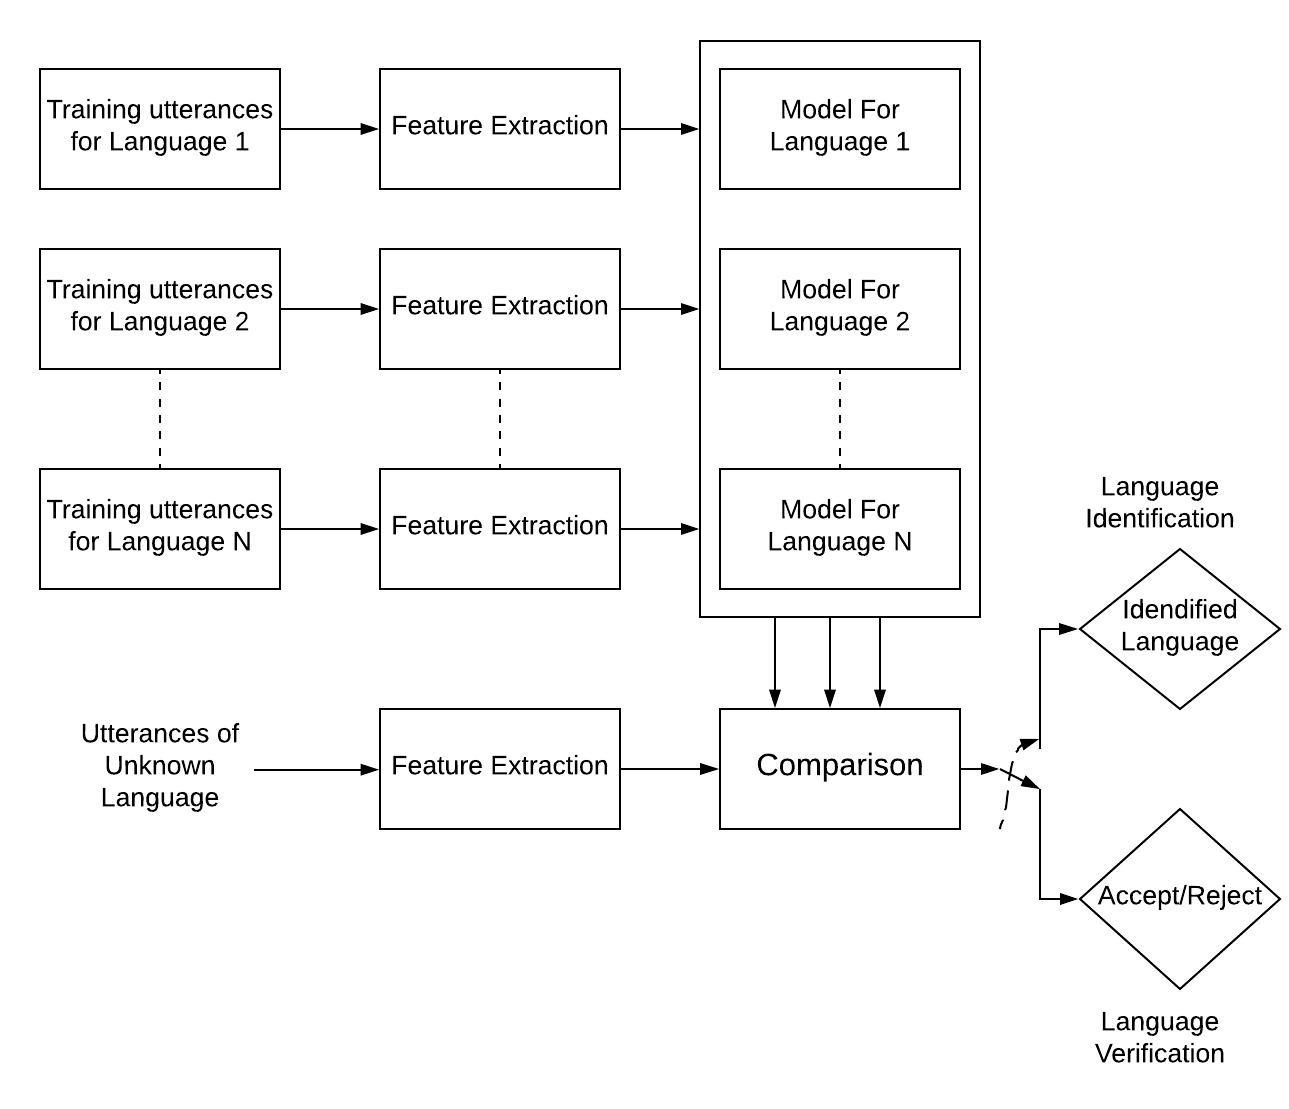
\includegraphics[scale=.65]{Images/lr.jpeg}}
\caption{Basic block diagram of language identification/verification system.}
\label{lr}
\end{figure} 
  
  Language recognition could be best manifested as a multiclass recognition problem, where the input belongs to one from the set of discrete classes. The objective is to recognize the class of the input. Let we have N target classes, $\{L_{1},L_{2},\ldots,L_{N}\}$. In the close-set there are N different specified languages, whereas in open set there are $N-1$ specified languages corresponds to $L_{1}, L_{2},\ldots, L_{N-1}$ target classes and  $L_{N}$ class denotes any unseen out of set languages. If $O$ is the spoken utterance
\begin{itemize}
    \item Language identification: Which of the N language does $O$ belongs to?
    \item Language verification: Does $O$ belongs to language $L_{l}$ or to other $N-1$ languages? 
\end{itemize}




\subsection{Language diarization}
Language diarization is a task to perform automatic language segmentation and recognition in a code-switched speech. Language diarization is different from language recognition, as in language recognition the test utterance is a monolingual utterance and the task is to identify the language identity. But in the case of language diarization, the test utterance's both the language identity and boundary of the language transition is unknown and the task is to find the language identity and language boundary. The basic block diagram of the language diarization system is shown in figure~\ref{ld}. The most challenging part of language diarization is the duration of mono-lingual segments of code-switched speech, which are much shorter than those traditionally studied in the language recognition. The performance of language diarization was measured in-terms of frame error rate (FER)~\cite{lyu2013language}. The application of language diarization can improve the performance of multilingual automatic speech recognition (ASR) system by improving the performance of Large vocabulary continuous speech recognition (LVCSR) when the test utterance contains code switch speech~\cite{lyu2013language}. Therefore for a country like India, where people use more than two languages while conversation, the language diarization system may play an important role to enhance the ASR performance.
 
 \begin{figure}[h]
\centering{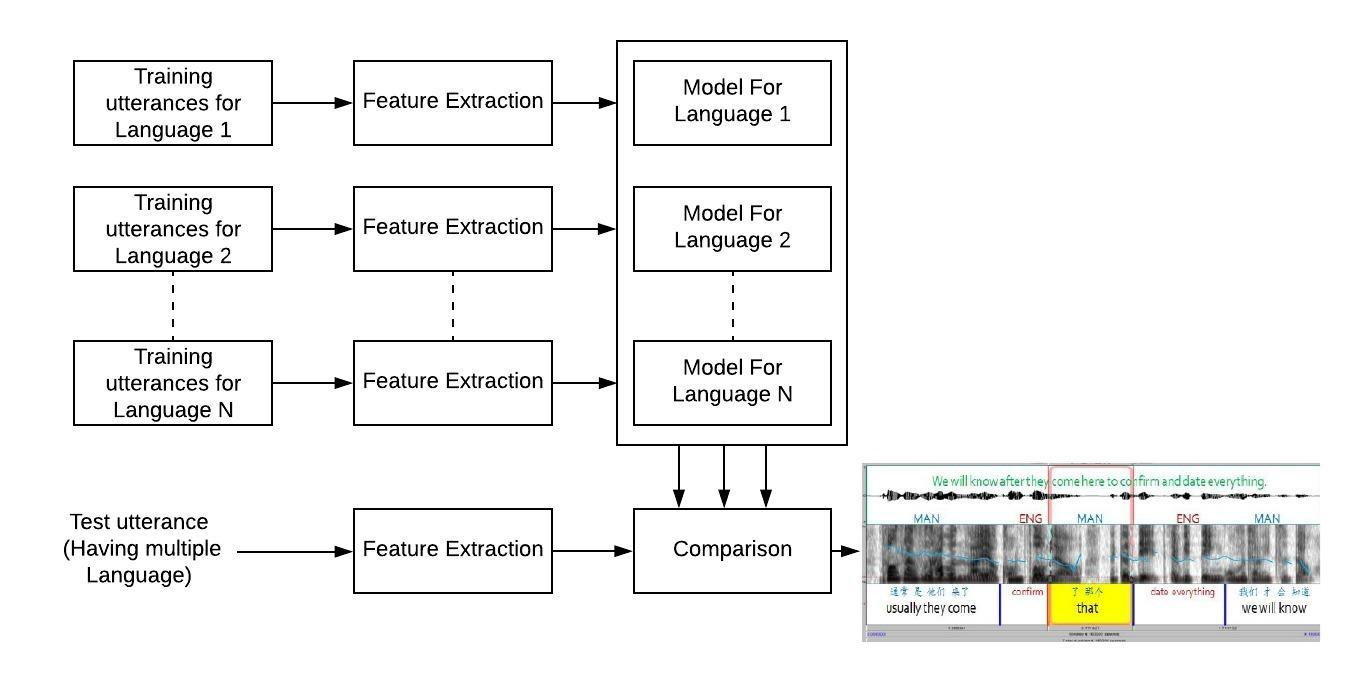
\includegraphics[scale=.65]{Images/language_diarization.jpeg}}
\caption{Basic block diagram of language diarization system~\cite{lyu2013language1}.}
\label{ld}
\end{figure} 
As like spoken language recognition, the language diarization can be performed by using both acoustic and phonotactic approach. In~\cite{lyu2013language}, Lyu et al. used 63-hour conversational South-East-Asia Mandarin/English (SEAME) code-switch corpus to perform language diarization experiment. In SEAME database, average language intervals in monolingual Mandarin and English segments are about 0.81 seconds and 0.67 seconds, respectively. The average number of language changes within a code-switched utterance is about $2.2$. They propose a phonotactic approach, where the acoustic features are passed through a phone recognizer and the phone recognizer output with different context was used to train a conditional random field (CRF) classifier. The performance of the system increases with increase in no of context frames. The best performance achieved was 14.4\% FER with context length $2$. In~\cite{yilmaz2017language}, Yilmaz et al. used an acoustic approach (BNF-UBM-I-vector) to perform language diarization. They use language diarization to perform automatic transcription of bilingual broadcast data. They observed that the use of language diarization with monolingual ASR instead of using bilingual ASR system improve the performance bilingual automatic transcription system. 
\section{Major milestones for language recognition}
The first attempt of identifying the spoken language was proposed in~\cite{leonard1974automatic}, where the phonotactic patterns were used to distinguish languages by computing the frequency of occurrence of certain sound units. To perform the language identification task they used five different languages and achieved an overall accuracy of 64\%. In the next attempt~\cite{house1977toward}, Markov process was used to model the sequence of sounds having a manual transcription of the utterances of eight different languages. The next attempt was coming on 1980~\cite{li1980statistical}, where they modeled the real speech data using a Markov process with broad phone classes of five different languages and obtained a testing accuracy of 80\%. 

In 1982 Cimarusti et al.~\cite{cimarusti1982development} first time extracted acoustic features from the speech signal and modeled using a polynomial classifier. In this work they derived 100 features (i.e 15 area functions, 15 auto-correlation coefficients, 5 bandwidths, 15 Cepstral coefficients, 15 filter coefficients, 5 formant frequencies, 15 log area ratios, and 15 reflection coefficients) from the linear prediction coefficient of the speech utterance having frame size 30 msec with a context shift of 30 msec. They used 8 languages in the study and achieved an accuracy of 84\%. In~\cite{foil1986language}, Foil et al. used noisy radio recordings to identify the languages, where they examined two types of language identification systems. In the first approach, they extracted seven prosodic features (based on rhythm and intonation) from pitch and energy contour. In the second they used formant frequencies (in terms of values and locations) to represent the characteristic sound patterns of the language. A k-means clustering algorithm and VQ were used for classification. The language identification performance achieved on three languages was 64\% correct with 11\% rejection on the test data duration of 4.5 seconds with the signal to noise ratio (SNR) of 5 dB. Motivating by the work of Foil et al., In~\cite{goodman1989improved} Goodman et al. attempted to improve the LPC based format extraction algorithm with six language database and test data duration of smaller than 10 seconds. The final performance was reported in terms of, a function of time, SNR and no-decision rate. 

In~\cite{sugiyama1991automatic}, Sugiyama et al. performed VQ classification on LPC derived features. They explored the difference between using one VQ codebook per language vs. one common VQ codebook for all languages, where the languages were classified according to their occurrence probability in histogram patterns. The experiment results show that the recognition rates for the first and second algorithms were 65\% and 80\%, respectively. The speech database used in this paper contains 20 languages: 16 sentences uttered twice by 4 males and 4 females with a duration of 8 seconds each.

In~\cite{nakagawa1992speaker}, Nakagawa et al. compared four methods VQ, discrete HMM, continuous density HMM and GMM. Comparative analysis of all mentioned methods was conducted in four languages. In the final performance, it is shown that the results obtained using continuous HMM and GMM (81.1\%) were better than vector quantization (77.4\%) and discrete HMM (47.6\%).

In~\cite{zissman1993automatic}, Zissman et al. perform a comparative study using HMM and GMM as a classifier with standard MFCC features along with their delta coefficients. The algorithms were evaluated on four multi-language speech databases: a three language subset of the spoken language library, a three language subset of a five-language Rome laboratory database, the 20 language CCITT database, and the ten languages OGI telephone
speech database~\cite{muthusamy1992ogi}. They observed that performance of single state HMM (I.e. GMM) classifier is comparable with the performance of multi-state HMM. The authors mentioned that the observed result may be due to the lack of training data to train the multi-state HMM. 

In~\cite{zissman1996comparison}, Zissman et al. compared the performance of four approaches for automatic spoken language identification. The approaches taken by them are  GMM for acoustic feature classification, single-language phone recognition followed by language-dependent interpolated n-gram language modeling (PRLM), parallel PRLM (which uses multiple single-language phone recognizer, each trained in a different language), and language dependent parallel phone recognition (PPR). The approaches were evaluated with the OGI multi-language telephone speech corpus and NIST 1994 corpus. They observed the systems have phone recognizer performed better than the GMM classifier. The top-performing system was parallel PRLM, which exhibited an error rate of 2\% for 45-s utterances and 5\% for 10-s utterances in two-language, closed-set, forced choice
classification. The error rate for 11-language, closed-set, forced-choice classification was 11\% for 45-s utterances and 21\% for 10-second utterances.

In~\cite{wong2002methods}, the authors used GMM-universal background model (UBM) classifier in the spoken language recognition task, by motivating the performance of GMM-UBM over standard GMM in speaker recognition~\cite{reynolds2000speaker}. They used 39 dimensions MFCC features along with its velocity and acceleration coefficients with vocal tract length normalization (usually use to suppress speaker dependent information). They used GMM-UBM classifier, to model the acoustic feature vectors. They observed the performance of GMM-UBM is better (i.e 13.4\%) than Parallel PRLM approach (i.e 16.6\%) in case of 45 sec testing case, but in the case of 10 sec testing case the performance of parallel PRLM (PPRLM) (i.e 24.8\%) is better than the GMM-UBM based approach (i.e 27\%). The overall fused system performance is 10.2\% for 45 sec and 18.4\% for the 10-sec testing case. They used OGI Multi-Language Telephone Speech Corpus and NIST 1994 corpus for conducting experiments.

In~\cite{torres2002approaches}, they were motivated by the performance of multiple-language phone recognition and n-gram language modeling on language identification task, which indicates that the automatic language identification task largely depends on the sequence information of speech utterances. The standard MFCC features are not able to capture sequence information of the utterances. In this paper they used shifted delta coefficient (SDC) which captured sequence information of speech utterances. They observed that the results obtained are comparable with phonotactic based PPRLM method. They used CallFriend and OGI corpora for system evaluation and achieved the best performance of 6.90\% in CallFriend corpora.


In~\cite{li2007vector}, they proposed a vector space modeling (VSM) method for automatic spoken language identification (LID) by motivating that the overall sound characteristics of all spoken languages can be covered by a universal collection of acoustic units, which can be characterized by the acoustic segment models (ASMs). A spoken utterance is then decoded into a sequence of ASM units. The ASM framework furthers the idea of language-independent phone models for LID by introducing an unsupervised learning procedure to circumvent the need for phonetic transcription. This is analogous to representing a text document as a term vector.  They converted a spoken utterance into a feature vector with its attributes representing the co-occurrence statistics of the acoustic units, then built a vector space classifier for LID. The proposed VSM approach leads to a discriminative classifier at the back-end. The observed result tells that the latter approach gives superior performance over likelihood-based n-gram language modeling (LM) back-end for long utterances. The performance of the proposed VSM framework in-terms of equal error rate (EER) was 2.75\% and 4.02\% in the 1996 and 2003 NIST language recognition evaluation (NIST-LRE) 30-second tasks, respectively.

In~\cite{ma2007spoken}, they used an ensemble of binary classifiers with shifted delta coefficient (SDC) to perform spoken language recognition. They adopted a distributed output coding strategy in ensemble classifier design, where they decomposed a multiclass language recognition problem into many binary classification tasks, each of which addresses a language recognition sub-task by using a component classifier. Then, they combined the results of the component classifiers to form an output code as a hypothesized solution to the overall language recognition problem. In this way, they effectively projected the high-dimensional feature vectors into a low-dimensional space by maintaining language discriminating characteristics of the spoken utterances. By fusing the output codes from both phonotactic features and cepstral features, they achieved an equal-error-rates of 1.38\% and 3.20\% for 30-second trials on the 2003 and 2005 NIST-LRE databases respectively.



In~\cite{dehak2011language}, motivated by the improvement in performance of speaker recognition system using I-vector based modeling, the authors use I-vector based modeling approach in spoken language recognition task. They achieved a performance of 2.1\% EER on NIST 2009 evaluation protocol.

In~\cite{song2013vector}, i-vector representation based on BNF features is presented for language identification (LID). In the proposed system, the BNF features are extracted from a deep neural network, which can effectively mine the contextual information embedded in speech frames. The i-vector representation of each utterance is then obtained by applying a total variability approach to the BNF features. The resulting performance of the LID has been significantly improved with the proposed BNF feature based i-vector representation. The obtained best result was 1.98\%, 3.47\%, 9.71\% in-terms of EER  on the NIST 2009 evaluation set with 30, 10 and 3 seconds test duration respectively.

In~\cite{gonzalez2014automatic}, they explore the use of Long Short-Term Memory (LSTM) recurrent neural networks (RNNs) for automatic language identification (LID). The use of RNNs is motivated by their better ability in modeling sequences with respect to feedforward networks. From the work, it is observed that long short term memory (LSTM) RNNs can effectively exploit temporal dependencies in acoustic data and learn relevant features for language discrimination. The proposed approach is compared to baseline i-vector and feedforward Deep Neural Network (DNN) systems in the NIST Language Recognition Evaluation 2009 dataset. The work shows LSTM RNNs achieve better performance than feedforward net based DNN system and i-vector system. The performance using LSTM RNN was 8.35\% in terms of average EER with 3-second test data, which is better compared to 9.58\% in feedforward net with 8 layers and 15.89\% in I-vector system. 

In~\cite{lei2014application}, they used a convolutional neural network (CNN) for the training of automatic speech recognition (ASR) system, the posterior of the model is used for i-vector extraction instead of UBM posteriors. The task was performed on the RATS database with five target languages (Farsi, Urdu, Pashto, Arabic, Levantine, and Dari) and achieved a performance of 10.95\%, 5.24\% and 3.53\% with 30, 10 and 3 seconds test utterances respectively. 

In~\cite{richardson2015deep}, Richardson et al. compared standard i-vector and various deep learning approaches for spoken language recognition task. Motivated by the gain of performance in ASR by using deep learning frameworks, the authors used deep feedforward network as a classifier, phonetic aware deep feedforward network for i-vector computation and bottleneck features were extracted from a deep feedforward network, which is used later to model the i-vector. Finally, it is observed that the performances of bottleneck feature (BNF) based i-vector system outperform the performances of all other systems. In NIST 2011 language recognition evaluation set the best performance achieved in-terms of $C_{avg}$ was 0.304\% using DNN as posterior in 30 seconds, 1.24\% in 10 seconds and 7.53\% in 3 seconds using GMM as posterior with BNF-i-vector system.     


In~\cite{zhang2018language}, Zhang et al. mentioned that traditional bottleneck feature extraction requires additional transcribed speech information, which is very difficult to get. Hence they proposed alternate unsupervised deep learning methods for bottleneck feature extraction. They used unsupervised cluster Gaussian mixtures for posterior labeling of frames instead of using posterior phone labeling for bottleneck feature extraction. They also used variational autoencoder and adversarial autoencoder for speech feature extraction. Then they used the i-vector framework to classify spoken languages. In this work they use three databases: 1) a four Chinese dialect dataset, 2) a five Arabic dialect corpus, and 3) multigenre broadcast challenge corpus (MGB-3) for language recognition task. The best fusion system performance archived in Chinese dataset was 95.7\% accuracy, in Pan-Arabic was 81.3\% accuracy and in MGB-3 dataset was 65.4\% accuracy.

In~\cite{snyder2018spoken}, Snyder et al. applied x-vectors to the task of spoken language recognition motivated by the performance of x-vector in the speaker recognition task. The x-vector framework consists of a deep neural network that maps sequences of speech features to fixed-dimensional embeddings, called x-vectors. In this framework, long-term language characteristics are captured in the network by a temporal pooling layer that aggregates information across time. Once x-vectors were computed, the same classification procedure like i-vectors was followed. In 2017 NIST-LRE, x-vectors outperformed all state-of-the-art i-vector systems. The best performance achieved using x-vectors (multilingual BNF with augmentation) in terms of $c_{avg}$ was 14.0\% in 3 seconds of test data.

The summary of all the works reported above towards spoken language recognition is tabulated in table~\ref{tab_review} and table~\ref{tab_review2}.

\begin{table}
\caption{A summary on different studies made on language recognition.}
\label{tab_review}
\begin{tabular}{|l|l|l|l|}
\hline
LRE Systems         & Method used                                                                                          & Performance                                                                                                                 & Database                                                                                                \\ \hline
Leonard et al.~\cite{leonard1974automatic}      & Phonotactic Pattern                                                                                  & \begin{tabular}[c]{@{}l@{}}Identification \\ accuracy=64\%\end{tabular}                                                     & \begin{tabular}[c]{@{}l@{}}In house data \\ (five language)\end{tabular}                                \\ \hline
House et al.~\cite{house1977toward}        & \begin{tabular}[c]{@{}l@{}}Markov Process\\ (Manual phone\\ transcription)\end{tabular}              &                                                                                                                             & \begin{tabular}[c]{@{}l@{}}In house data\\ (Eight language)\end{tabular}                                \\ \hline
Li et al.~\cite{li1980statistical}           & \begin{tabular}[c]{@{}l@{}}Markov Process\\ (Real speech model)\end{tabular}                         & \begin{tabular}[c]{@{}l@{}}Identification \\ accuracy=80\%\end{tabular}                                                     & \begin{tabular}[c]{@{}l@{}}In house data \\ (Five language)\end{tabular}                                \\ \hline
Cimarusti et al.~\cite{cimarusti1982development}    & \begin{tabular}[c]{@{}l@{}}100 dimension \\ acoustic feature\\ (Polynomial Classifier)\end{tabular} & \begin{tabular}[c]{@{}l@{}}Identification \\ accuracy=84\%\end{tabular}                                                     & \begin{tabular}[c]{@{}l@{}}In house data\\ (Eight language)\end{tabular}                                \\ \hline

Foil et. al.~\cite{foil1986language}        & \begin{tabular}[c]{@{}l@{}}Prosodic feature,\\ Frequency of\\ Format location\end{tabular}           & \begin{tabular}[c]{@{}l@{}}Identification \\ accuracy=64\%\end{tabular}                                                     & \begin{tabular}[c]{@{}l@{}}In house data,\\ Noisy data\\ with 5 dB SNR\\ (Three language)\end{tabular} \\ \hline
Goodman et al.~\cite{goodman1989improved}      & \begin{tabular}[c]{@{}l@{}}Improved LPC based\\ Format extraction\\ algorithm\end{tabular}          &                                                                                                                             & \begin{tabular}[c]{@{}l@{}}In house data,\\ Noisy data\\ (Six language)\end{tabular}                   \\ \hline
Sugiyama et al.~\cite{sugiyama1991automatic}     & \begin{tabular}[c]{@{}l@{}}LPC derive feature\\ VQ Code-book\end{tabular}                             & \begin{tabular}[c]{@{}l@{}}Identification \\ accuracy=80\%\end{tabular}                                                     & \begin{tabular}[c]{@{}l@{}}In house data,\\ (Twenty language)\end{tabular}                              \\ \hline
Nakagawa et al.~\cite{nakagawa1992speaker}    & \begin{tabular}[c]{@{}l@{}}VQ,\\ Discrete HMM,\\ Continuous HMM,\\ GMM\end{tabular}                  & \begin{tabular}[c]{@{}l@{}}Identification \\ accuracy=81.1\%\end{tabular}                                                   & \begin{tabular}[c]{@{}l@{}}In house data,\\ (Four language)\end{tabular}                                \\ \hline
Zissman et al.~\cite{zissman1993automatic}     & \begin{tabular}[c]{@{}l@{}}HMM,\\ GMM\\ (MFCC+ Delta)\end{tabular}                                   &                                                                               \begin{tabular}[c]{@{}l@{}}Identification \\ accuracy=80\%\end{tabular}                                              & OGI-11L Data set                                                                                        \\ \hline
Zissman et al.~\cite{zissman1996comparison}      & \begin{tabular}[c]{@{}l@{}}GMM\\ Parallel PRLM\end{tabular}                                          & \begin{tabular}[c]{@{}l@{}}Error rate\\ 45 sec- 11\%\\ 10 sec- 21\%\end{tabular}                                            & \begin{tabular}[c]{@{}l@{}}OGI-11L Data set\\ NIST 1994\end{tabular}                                                                                                                                   \\ \hline
Wong et al. ~\cite{wong2002methods}         & GMM-UBM                                                                                              & \begin{tabular}[c]{@{}l@{}}Error rate\\ 45 sec- 10.2\%\\ 10 sec- 18.4\%\end{tabular}                                        & \begin{tabular}[c]{@{}l@{}}OGI-11L Data set\\ NIST 1994\end{tabular}                                    \\ \hline
Carrasquillo et al.~\cite{torres2002approaches} & \begin{tabular}[c]{@{}l@{}}SDC-GMM,\\ PPRLM\end{tabular}                                             & \begin{tabular}[c]{@{}l@{}}Error rate\\ 45 sec- 6.90\%\end{tabular}                                                         & \begin{tabular}[c]{@{}l@{}}OGI  Data set\\ CallFriend Corpus\end{tabular}                               \\ \hline
Li et al.~\cite{li2007vector}           & \begin{tabular}[c]{@{}l@{}}Vector Space\\ Modelling (VSM)\end{tabular}                               & \begin{tabular}[c]{@{}l@{}}EER\\ 30 sec- 2.75\% (1996)\\ 30 sec- 4.02\% (2003)\end{tabular}                                 & \begin{tabular}[c]{@{}l@{}}NIST-1996\\ NIST-2003\end{tabular}                                           \\ \hline


\end{tabular}
\end{table}



\begin{table}[ht]
\caption{A summary on different studies made on language recognition.}
\label{tab_review2}
\begin{tabular}{|l|l|l|l|}
\hline
LRE Systems         & Method used                                                                                          & Performance     & Database    \\ \hline
  Ma et al.~\cite{ma2007spoken}           & \begin{tabular}[c]{@{}l@{}}SDC\\ Binary Classification\end{tabular}                                   & \begin{tabular}[c]{@{}l@{}}EER\\ 30 sec- 1.38\% (2003)\\ 30 sec- 3.20\% (2005)\end{tabular}                                 & \begin{tabular}[c]{@{}l@{}}NIST-2003\\ NIST-2005\end{tabular}  \\ \hline                                                                                                       
                                         
Dehak et al.~\cite{dehak2011language}        & I-vector                                                                                             & \begin{tabular}[c]{@{}l@{}}EER\\ 30 sec-2.1\%\end{tabular}                                                                  & NIST-2009                                                                                               \\ \hline
Song et al.~\cite{song2013vector}         & BNF-I vector                                                                                         & \begin{tabular}[c]{@{}l@{}}EER\\ 30 sec-1.98\%\\ 10 sec-3.47\%\\ 3 sec-9.71\%\end{tabular}                                  & NIST-2009                                                                                               \\ \hline
Gonzalez et al.~\cite{gonzalez2014automatic}     & RNN-LSTM                                                                                             & \begin{tabular}[c]{@{}l@{}}EER\\ 3 sec- 8.35\%\end{tabular}                                                                 & NIST-2009                                                                                               \\ \hline
Lei et al.~\cite{lei2014application}          & CNN-I vector                                                                                         & \begin{tabular}[c]{@{}l@{}}EER\\ 30 sec- 10.95\%\\ 10 sec- 5.24\%\\ 3 sec-3.53\%\end{tabular}                               & \begin{tabular}[c]{@{}l@{}}RATS\\ (Five language)\end{tabular}                                          \\ \hline


Richardson et al.~\cite{richardson2015deep}   & \begin{tabular}[c]{@{}l@{}}DNN\\ DNN-I-Vector\\ BNF-UBM-I-vector\\ BNF-DNN-I-vector\end{tabular}       & \begin{tabular}[c]{@{}l@{}}$C_{avg}$\\ 30 sec-0.304\%\\ 10 sec-1.24\%\\ 3 sec- 7.53\%\end{tabular}                               & NIST-2011                                                                                               \\ \hline
Zhang et al.~\cite{zhang2018language}        & \begin{tabular}[c]{@{}l@{}}Unsupervised BNF\\ Autoencoder Feature\end{tabular}                       & \begin{tabular}[c]{@{}l@{}}Identification\\ accuracy\\ Chinese - 95.7\%\\ Pan Arabic - 81.3\%\\ MGB-3 - 65.4\%\end{tabular} & \begin{tabular}[c]{@{}l@{}}Chinese Dialect\\ Pan Arabic\\ MGB-3\end{tabular}                           \\ \hline
Snyder et al.~\cite{snyder2018spoken}       & X-vector                                                                                             & \begin{tabular}[c]{@{}l@{}}$C_{avg}$\\ 3 sec - 14.0\%\end{tabular}                                                             & NIST-2017                                                                                               \\ \hline

\end{tabular}
\end{table}


\section{Databases for spoken language recognition}
The availability of large dataset has been the major driving factor in the development of speech technology~\cite{li2013spoken}. To design a spoken language recognition system, we need a set of speech data of different languages having variations within the language like intersession variability, speaker variation, device variation and recording environment variation. 

There are three standard organizations, who develop standard challenge databases for language recognition study. These standard corpora are Oregon graduate institute telephone speech corpus(OGI-TS), LDC call friend telephone speech corpus and NIST Language recognition corpus.

\subsection{Oregon graduate institute telephone speech corpus (OGI-TS)}
The OGI-TS is the first publicly available multi-lingual speech corpus developed to perform spoken Language recognition task~\cite{muthusamy1992ogi}. The OGI-TS speech corpus contains the speech from 11 languages: English, Farsi, French, German, Hindi, Japanese, Korean, Mandarin, Chinese, Spanish, Tamil, and Vietnamese. Each language contains the speech from about 80 native speakers, where each speech utterance in the corpus was spoken by a unique speaker over the telephone channel with a sampling frequency of 8kHz. The corpus was collected and developed in 1992, and the latest version was released in 2002 which includes recorded utterances from about 2052 speakers, for a total of about 38.5 hours of speech.
\subsubsection{OGI-TS 22 language corpus}
The current version of the OGI 22 Language corpus consists of telephone speech from 21 languages: Arabic, Cantonese, Czech, English, Farsi, German, Hindi, Hungarian, Japanese, Korean, Indonesian, Mandarin Chinese, Italian, Polish, Portuguese, Russian, Spanish, Swedish, Swahili, Tamil and Vietnamese~\cite{lander1995ogi}. The corpus contains fixed vocabulary utterances (e.g. days of the week) as well as fluent continuous speech. Approximately 20,000 utterances in 16 languages have corresponding orthographic transcriptions.


\subsection{LDC callfriend telephone speech corpus}
The call friend corpus released by LDC having unscripted conversion speech of 12 languages~\cite{ambikairajah2011language,li2013spoken}. These 12 languages are Egyptian Arabic, English, Farsi, French, German, Hindi, Japanese, Korean, Mandarin, Spanish, Tamil, and Vietnamese. From the 12 languages, 3 languages each having two dialects: English (American English with southern and non-southern dialect ), Mandarin (Mainland and Taiwan dialect), Spanish (Spanish-Caribbean and Spanish-Non Caribbean dialect). Dialect means the variation in utterances of the same language by the speakers belongs to the different geographical region. The database consists of 60 telephone conversations for each language, where 20 are used for the training set, 20 for the development set and 20 for the evaluation set. As per the protocol the training set is used to train the language model and classifier, the development set to train the back-end classifier and the evaluation set for final system evaluation.   
\subsection{NIST Language recognition corpus (NIST LRE)}
The National Institute of Standards and Technology (NIST) has conducted a series of evaluations of spoken language recognition in 1996, 2003, 2005, 2007, 2009, 2011, 2015 and 2017~\cite{martin2003nist,martin2009,greenberg20122011}.These  evaluations  have  been designed  to  foster  research progress, with the goals of
\begin{enumerate}
    \item Exploring promising new ideas in language recognition.
    \item Developing advanced technology incorporating these ideas.
    \item Measuring the performance of this technology.
\end{enumerate}
It has been seen that more languages are added from year to year. The emphasis of NIST LRE has been on conversational telephone speech (CTS), since most of the likely applications of the technology involve signals recorded from the public telephone system. In order to collect speech data of more languages in a cost-effective way, NIST has adopted broadcast narrow-band speech (BNBS) lately in LRE 2009, LRE 2011, LRE 2015 and LRE 2017. BNBS data are excerpts of call-in telephone speech embedded in broadcast and webcast. The call-in excerpts are used as we could expect them to cover as many speakers as possible. Broadcast entities like the Voice of America (VOA) broadcast are having more than 45 languages. Alternatively, the British Broadcast Company (BBC) also produces and distributes programs in a large number of languages. The number of target languages in NIST 1996 has 12, NIST 2003 has 12, NIST 2005 has 9, NIST 2007 has 24 with 5 open-set languages, NIST 2009 has 23 with 16 open-set languages, NIST 2011 has 24, NIST 2015 has 20 and NIST 2017 has 14. In NIST 2017, unlike previous  LREs the evaluation data will be divided into partitions based on the data source, i.e., MLS14 and VAST, for each language, resulting in a total of 28 partitions. The NIST evaluation protocol has three testing conditions:
30 seconds, 10 seconds and 3 seconds.

\section{Performance measure for language recognition}

The spoken language recognition experiments generally evaluated by identification accuracy, average equal error rate, and average detection cost~\cite{li2013spoken}.

\subsection{Average detection cost($C_{avg}$)}
As per NIST LRE, the language recognition system performance is evaluated in terms of average detection cost. In spoken language recognition, the
performance is evaluated by presenting the system with a set of trials, each consisting of a test segment and a hypothesized target language. The system has to decide for each trail that whether the target language was spoken in the given segment.

Let $N_{T}$ be the number of test segments and $N$ be the number of target languages. By presenting each test segment against all target languages, there are $N_{T}$ number of trials for each target and the system under evaluation should produce $N \times N_{T}$ number of true or false
decisions. The average detection cost can be written as,
$$C_{avg}=\frac{1}{N}\sum_{l=1}^{N}C_{DET}(L_{l})$$
where $C_{DET}(L_{l})$ is the detection cost for the subset of $N_{T}$ trials for which the target language is $L_{l}$.
$$C_{DET}(L_{l})=C_{miss}P_{tar}P_{miss}(L_{l})+C_{fa}(1-P_{tar})\frac{1}{N-1}\sum_{m \neq l}P_{fa}(L_{l},L_{m})$$

where $C_{miss}$ and $C_{fa}$ are the cost of making false rejection (miss probability) and false acceptance. $P_{tar}$ is the prior probability of the target. In general $C_{miss}$, $C_{fa}$ and $P_{tar}$ are fixed to 1, 1 and 0.5 respectively. $P_{miss}$ is the false rejection probability and  $P_{fa}$ is the false acceptance probability. 





\section{Summery and Discussion}
The various key aspects of Automatic Language Recognition system are discussed in this report. It includes several key aspects of language recognition, covering language characterization and various modeling techniques useful in automatic language recognition. Various system development strategies regarding the task are also discussed. It has been seen from the literature that tremendous development is observed in language recognition in the last few decades. Incorporation of DNN technique in the field of language recognition dramatically change the performance of the system. Though the language recognition is still far from perfect. From the literature, it is observed that SDC features have better language discrimination ability than all the other available features. As SDC feature capture speech dynamics over a wide range of speech frames, which helps to capture some phonotactic information also. Before the incorporation of DNN based frameworks, SDC with i-vector framework was the state-of-art language recognition technique. After neural network based approaches evolved in the field of language recognition BNF based i-vector approach has been used as the state-of-the-art approach. Recently found that the x-vector framework, which was originally developed for speaker recognition, outperformed several state-of-the-art i-vector systems on the NIST LRE 2017 database in the language recognition task. The NIST LRE database series is the most widely used dataset for language recognition study.

It had been shown that acoustic and phonotactic features have been widely used in the language recognition task. Whereas human listening experiments indicated that prosodic and other high-level features are equally informative. This prompts us to develop some techniques for language recognition in the future, which can effectively capture such high-level information to further improve the performance of the system.





%\section{Background}
% \lettrine[lines=1]{\textbf{I}}{ntroduction} Introduction
% 
% \section{Section 1}
% "Section Description" ~\cite{Cite01}, "Section Description"
% \begin{equation}
% \label{eq1}
% x = y + z
% \end{equation}
% 
% Equation \ref{eq1} adds 2 numbers.
% 
% 
% \section{Section 2}
% "Section Description"
\end{spacing} 



\chapter{Acoustic feature extraction and classification techniques used for Spoken language recognition}
%\chaptermark{Acoustic feature extraction and classification techniques used for Spoken language recognition}
\HRule \\[-0.5cm] % Horizontal line

%\label{Chapter2} % For referencing the chapter elsewhere, use \ref{Chapter1}

%\lhead{\emph{\textbf{Chapter2:} Acoustic feature extraction and classification techniques used for Spoken language recognition}} % This is for the header on each page - perhaps a shortened title

%----------------------------------------------------------------------------------------
%	SECTIONS
%----------------------------------------------------------------------------------------
\begin{spacing}{1.5}
The acoustic information is generally considered as the first level analysis of speech production. Human speech is a longitudinal pressure wave, and different speech events can be distinguished at an acoustic level, according to amplitude and frequency components of the waves. The acoustic information is one of the simplest forms of information, which can be obtained during the speech parameterization process directly from raw speech. The higher level of speech information like phonotactic and word information can also be extracted from the acoustic information~\cite{ambikairajah2011language}. For the spoken language recognition task, the Mel frequency cepstral coefficients (MFCC) are the most widely used feature extraction technique. The language discriminative information largely reflects on the temporal patterns of the speech signal. Thus, once the basic acoustic features have been obtained, additional features are appended to each feature vectors. Some commonly utilized additional features are the delta and acceleration cepstrum (MFCC + delta + acceleration) and the shifted delta cepstrum (SDC).

\section{Mel frequency cepstral coefficients (MFCC)}
The Mel frequency cepstral coefficients (MFCCs) are one of the most commonly used filter-bank based parameterization method for speech processing applications, such as speech recognition, speaker verification/identification and spoken language recognition. The human perception of the frequency content of the sound follows a nonlinear scale called Mel scale~\cite{chakroborty2009improved}. So, the Mel-scale is used to approximate the nonlinear frequency resolution of the human ear. After the magnitude-square of the Fourier Transform is calculated for the input windowed frame of speech, it is passed through a bank of triangular Mel filters and the natural logarithm of the filter bank energies is taken. As the filter bank log-energies are highly correlated, a linear transformation technique (I.e the Discrete Cosine Transform (DCT)) is used to de-correlate the information yielding in Mel frequency cepstral coefficients. The steps to extract MFCC Features from speech sample is depicted in figure~\ref{mfcc}. The brief description of all the steps are as follows.
\begin{figure}[h]
\centering{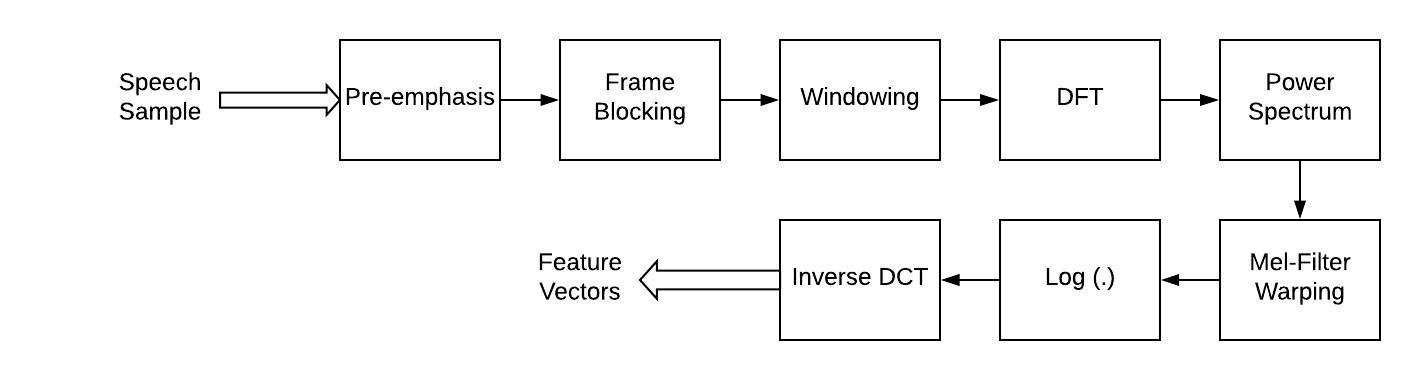
\includegraphics[scale=.55]{Images/mfcc.jpeg}}
\caption{Block diagram of MFCC extraction.}
\label{mfcc}
\end{figure} 
\subsection{Pre-emphasis}
\begin{figure}[h]
\centering{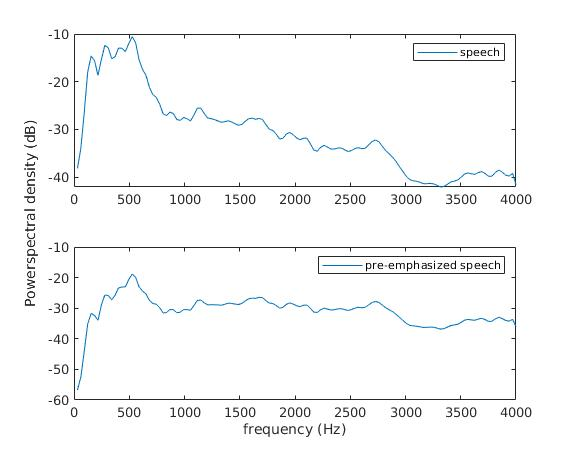
\includegraphics[scale=.55]{Images/pre_effect.jpg}}
\caption{The power spectral density of the original speech signal and pre-emphasized speech signal sampled at 8000 Hz.}
\label{pemp}
\end{figure} 
Figure~\ref{pemp} shows the power spectral density of the original speech and its pre-emphasized speech. It has been observed from the figure that the power of the signal falls sharply in high frequency regions. It is estimated that about 80\% of the power is contained within frequency components below 1000 Hz~\cite{beigi2011speaker}. To perform verious recognition task human ear's cochlea utilizes a fine-tuning mechanism based on feedback from the brain that amplifies special frequencies. Therefore the human ear can easily recognize these low energy regions. Since our objective is to design a recognition system, we have to do something to enhance the high frequency components, by which high frequency information can also play a role in recognition task. This can be achieved through pre-emphasis. One method which has been used quite often is a differentiator (single zero filter), whose transfer function is given in equation~\ref{pr}  


\begin{equation}
\label{pr}
    H_{p}(z)=1-\alpha z^{-1}
\end{equation}
The most popular range of values for $ \alpha $ is between 0.95 and 0.97, although values in the range of 0.9 and just less than 1.0 have also been used in different systems.
Figure~\ref{pemp} shows the power spectral density of the pre-emphasized signal using $ \alpha=0.98 $. Here we notice that the absolute power for each frequency range has been reduced, but the relative power is better distributed along the different frequencies.

\subsection{Frame blocking} The speech is slow varying quasi-stationary signal.
Therefore, speech analysis must always be carried out on short segments across which the speech signal is assumed to be stationary. Short-term spectral measurements are typically carried out over the range of 10-30 ms frame size and shift~\cite{beigi2011speaker}. In that direction, the speech signal is divided into frames of L samples, with adjacent frames being separated by M samples with the value M less than that of L. The first frame consists of the first L samples. The second frame begins from M samples after the first frame, and overlaps it by L - M samples and so on. This process continues until all the speech samples are taken into account.

\subsection{Windowing} The next step is to window each individual frame to minimize the signal discontinuities at the beginning and end of each frame. The concept applied here is to minimize the spectral distortion by using the window to taper the signal to zero at the beginning and end of each frame. If we define the window as w(n), $0 \leq n \leq L-1$  where L is the frame length, then the result of windowed signal can be written as:
\begin{equation}
 s_{o}(n)=w(n).s_{i}(n)
\end{equation} 
where w(n) the window function. In general hamming window (to eliminate the problem of spectral leakage and zero offset) is widely used to analyze the speech frames.


\begin{equation}
 w(n)=0.54-0.46cos\Bigg(\frac{2\pi n}{L-1}\Bigg), 0\leq n \leq L-1
\end{equation} 


\subsection{DFT} The next step in the processing of the speech data to be able to compute its spectral features is to take a Discrete Fourier Transform of the windowed data. The DFT is computed using equation~\ref{dft}. The DFT length L is always grater then the windowed speech segments length to avoid time aliasing.

\begin{equation}
 \label{dft}
 S(k)=\sum_{n=0}^{L-1}s(n).e^{\frac{-j2\pi kn}{L}}, 1 \leq k \leq L-1, 1 \leq n \leq L-1
\end{equation}


\subsection{Power spectrum}  The loudness is related with intensity of the signal, hence our goal is to convert it into a value that would represent loudness so that we may mimic human perception. Therefore, after the calculation of DFT of each windowed speech segment the power spectrum ($|{S(K)}|^2$) is calculated.


\subsection{Mel filter warping} The human auditory perception is based on a scale which is somewhat linear up to the frequency of 1000 Hz and then becomes close to logarithmic for the higher frequencies.  This was the motivation to use the Mel scale. It has been seen from the literature, that the 24 band filter bank is used to model the auditory system~\cite{beigi2011speaker}. The designed 24 Mel filter banks are presented in figure~\ref{Mel}. First the lowest and highest frequency is converted to Mel scale using equation~\ref{hz2mel}. The unity height triangular filters are uniformly spaced in Mel scale, so in Mel scale the difference between the lowest and highest frequency are uniformly divided into M (no of filter)+1 segments to find the center frequency of each filter. Then the center frequencies which are in Mel scale are converted to Hz scale using equation~\ref{Mel2hz}~\cite{chakroborty2009improved}. The triangular filter banks ($H_{m}(k)$) can be constructed using equation~\ref{trf}. $\{k_{c_{m}}\}_{m=1}^{M}$ are the center frequencies of the filter, $k_{c_{0}}$ and $k_{c_{M+1}}$  are the boundary frequencies in Hz scale (lowest and highest frequency). The output of the Mel filter bank can be computed using equation~\ref{sMel}. Where $H_{m}(k)$ is the filter bank function and M is the no of filter bank used.

\begin{figure}[ht]
\centering{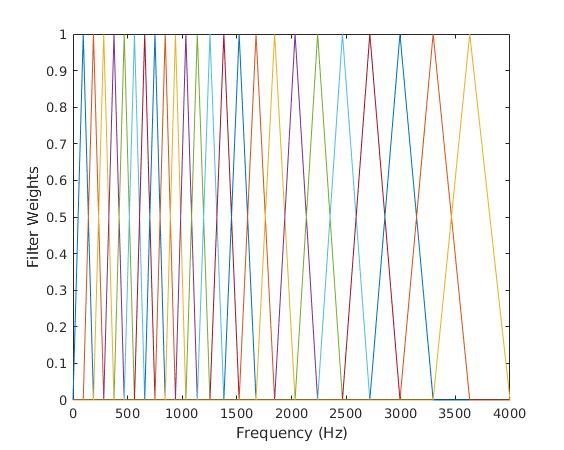
\includegraphics[scale=.35]{Images/mel.jpg}}
\caption{Shape of Mel filter bank for a 24 filter system with sampling frequency of 8000 Hz .}
\label{Mel}
\end{figure} 

\begin{equation}
f_{Mel}=2595 ~.~ log_{10}\Big(1+\frac{f_{lin}}{700}\Big)
%f=f_{high}+f_{low}-f_{Mel2hz}[f_{Mel}(f_{high})+f_{Mel}(f_{low})-f_{Mel}(f)]
\label{hz2mel}
\end{equation}

\begin{equation}
f_{lin}=700.\Big(10^{\frac{f_{mel}}{2595}}-1\Big)
%f=f_{high}+f_{low}-f_{Mel2hz}[f_{Mel}(f_{high})+f_{Mel}(f_{low})-f_{Mel}(f)]
\label{Mel2hz}
\end{equation}

\begin{equation}
H_{m}(k) =
\begin{cases}
0 & \text{for $k \leq k_{c_{m-1}}$}\\
\frac{k-k_{c_{m-1}}}{k_{c_{m}}-k_{c_{m-1}}} & \text{for $k_{c_{m-1}} \leq k \leq k_{c_{m}}$} \\
\frac{k_{c_{m+1}}-k}{k_{c_{m+1}}-k_{c_{m}}} & \text{for $k_{c_{m}} \leq k \leq k_{c_{m+1}}$} \\
0 & \text{for $k \geq k_{c_{m+1}}$}, \quad 1 \leq m \leq M
\end{cases}
\label{trf}
\end{equation}

\begin{equation}
 \label{sMel}
 S(m)=\sum_{k=1}^{N}|S(k)|^{2}H_{m+1}(k), 0 \leq m \leq M-1
\end{equation}



\subsection{log(.)} 
Now we have to warp the power spectra into a logarithmic scale. As we know the dynamic range of the power spectra very high in between different Mel frequency bands, so logarithm with base 10 is used to reduce the dynamic range. It has been seen that in human perception, the vocal tract response information plays a vital role to recognize speaker and language. In time domain the vocal tract response and excitation response are convoluted, therefore in frequency domain they are multiplied. The use of log(.), converts multiplication to addition, latter low time liftering is used to enhance the vocal tract information.    
\subsection{Inverse DCT}
In the previous section we computed the log of the power spectral density of the signal in Mel scale. By taking inverse discrete cosine transform (DCT), we will get the cepstrum of the signal. The most attractive features of the cepstrum is its inherent invariance toward linear spectral distortions, which make it a good candidate for usage in speaker and language recognition task. We can also compute the cepstrum using inverse discrete Fourier transform, but in that case the coefficients are complex (s(m) is not symmetric). One possibility is to take square magnitude of the coefficients or to use inverse DCT directly to get real coefficients. The coefficients using inverse DCT is computed using equation~\ref{dct}.     

\begin{equation}
 \label{dct}
 c(n)=\sum_{m=0}^{M-1}a_{m}log_{10}(S(m))cos\Bigg(\frac{\pi n(m-0.5)}{M}\Bigg), 0 \leq n \leq C-1
\end{equation}


    $$ a_{m}=
   \begin{cases}
    \frac{1}{M} & \text{for $m=0$} \\
     \frac{2}{M} & \text{for $m > 0$}
   \end{cases}$$

Where C is the no of cepstral coefficients needs to be computed and DCT length M should be always grater then or equal to the no of filter bank used to compute Mel coefficients.

\section{Delta and Delta-Delta cepstra ($\Delta$ and $\Delta-\Delta$)}

The static MFCC feature vectors provides a good estimation of local spectra, but it fails to capture the dynamics of human speech. The dynamics of human speech is very important information for distinguishing different     languages~\cite{ambikairajah2011language}.  Therefore, the performance of the system greatly enhanced by adding time derivative of basic static parameters. The Delta and Delta-Delta provides an estimation of local temporal derivatives of the speech cepstrum, and are implemented as a least square approximation of the local slope and calculated over multiple frames. The first order derivative are computed as delta coefficients and can be computed as per equation~\ref{del}.

\begin{equation}
\label{del}
    \Delta c_{i}(n)=\frac{\sum _{k=-N}^{k=N}kc_{i}(n+k)}{\sum _{k=-N}^{k=N}k^2}
\end{equation}
Where $\Delta c_{i}(n)$ is the delta coefficient of the $i^{th} $ cepstral stream and $n^{th} $ frame. The N defines the no of frames to be used for the computation of delta coefficients. Typically the range of N is from 2 to 4. Similarly the $\Delta-\Delta$ coefficients are computed using the same equation on Delta coefficients instead of static coefficients. As the Delta and Delta-Delta coefficients computation needs the coefficients of previous and post frame, needs some modification at beginning and end of speech. This end-effect
problem can be solved by using simple first order differences at the start and end of the speech (as per equation ~\ref{start} and ~\ref{end}).
\begin{equation}
\label{start}
    \Delta c_{i}(n)=c_{i}(n+1)-c_{i}(n),\quad n < N
\end{equation}
\vspace{-0.5 cm }
\begin{equation}
\label{end}
    \Delta c_{i}(n)=c_{i}(n)-c_{i}(n-1),\quad n \geq T-N
\end{equation}
Where T is the total no of frames. In general the delta and delta-delta cepstrum are concatenated with the static cepstrum to form a single
feature vector containing both the static and dynamic
information of the speech signal.

\section{Shifted delta coefficients (SDC)}
The delta and delta-delta feature able to capture the temporal information, But it is limited, and not able to capture the higher level temporal dynamics information. If we consider $N=2$, the delta and delta-delta can able to capture the temporal dynamics information across 5 frames, i.e. across 50 ms (if $frameshift=10 ms$).

Temporal information has proven useful in distinguishing languages, i.e accessing the likelihood of one phone following another (phonotactic information). Thus, this intuition leads to design a feature, which can capture the temporal dynamics information in a larger window. One way, we can choose larger N value in the delta calculations to include a much longer window in the calculation. But, this will only produce a much longer average of the slope and the finer details will be lost. The SDC feature is a better alternative to capture spectral dynamics in a longer window~\cite{torres2002approaches}. The SDC feature is obtained by concatenating future and past frames delta cepstra with the current feature vector.

In general, the computation of SDC are specified by four parameters: z, d, p, k. z specifies the number of basic cepstral streams to use in the calculation, i.e. the number of basic cepstral coefficients. Each of z cepstral streams are treated separately and SDC values are computed for each of them prior to concatenation with the original cepstral coefficients. p is the number of frames from one delta calculation to the next and k is the total number of delta values concatenated together to form the SDC. The diagram showing the computation procedure of SDC is shown in figure~\ref{sdc}

\begin{figure}[h]
\centering{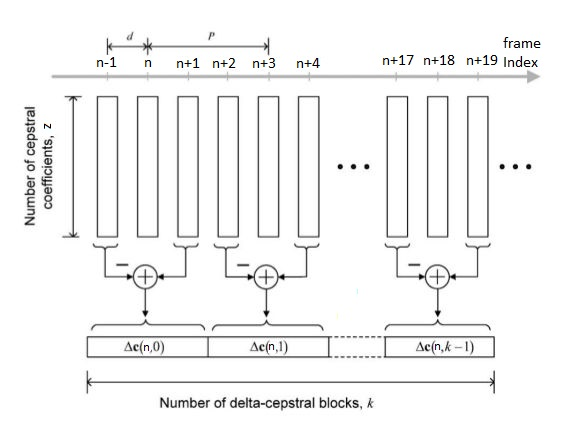
\includegraphics[scale=.55]{Images/sdc.jpg}}
\caption{SDC feature extraction at $n^{th}$ frame, $z-d-p-k=7-1-3-7$.}
\label{sdc}
\end{figure} 
The final parameter d is the difference value used in the delta calculation. for all the SDC calculations the delta values were calculated by subtracting the cepstral value at $n-d$ from that at $n+d$. Thus for each of the M cepstral streams, the final vector at time n is given by the concatenation of all the $\Delta c_{i}(n,z)$ for $0 \leq z \leq k$, where i represents the $i^{th}$ cepstral coefficient. The mathematical equation for the computation of $\Delta c_{i}(n,z)$ is given in equation~\ref{sdc1}.
\begin{equation}
    \label{sdc1}
    \Delta c_{i}(n,z)= c_{i}(n+zp+d)-c_{i}(n+zp-d)
\end{equation}
It has been seen that, the regression based delta computation is more efficient for better estimate then the method of simple subtracting~\cite{ambikairajah2011language}. In this way, the $\Delta c_{i}(n,z)$ can be computed using equation~\ref{sdc2}. 
\begin{equation}
\label{sdc2}
    \Delta c_{i}(n,z)=\frac{\sum _{l=-d}^{l=d}l c_{i}(n+zp+l)}{\sum _{l=-d}^{l=d} l^2}
\end{equation}
With either the standard subtraction method, or the modified regression based technique, the SDC capture temporal dynamics information in a much larger window then the standard delta and delta-delta. In general, people use SDC feature for language recognition task with configuration $z-d-p-k=7-1-3-7$. The best way to compute the SDC feature is, after computing static MFCC (c(n)) and its delta coefficients (d(n)), the SDC coefficients of the $n^{th}$ frame is given as: $$sdc(n)=\Big[c(n), d(n-p),\ldots,d(n),\ldots(d(n+p)) \Big ] $$ 

\section{Gaussian Mixture Model}
\label{gmm_sc}
Gaussian Mixture Model (GMM) is a parametric probability density function represented as a weighted sum of Gaussian component densities. GMMs are capable of representing a large class of sample distributions. Thus, GMMs are commonly used as a parametric model of the probability distribution of continuous measurements or features in a speaker and language recognition systems. 

The use of GMM may also be motivated by the intuitive notion that the individual component densities may model some underlying set of hidden classes. For example, in speaker recognition, it is reasonable to assume the acoustic space of spectral related features corresponding to a speaker’s broad phonetic events, such as vowels, nasals or fricatives. These acoustic classes reflect some general speaker dependent vocal tract configurations that are useful for characterizing speaker identity. The spectral shape of the $i^{th}$ acoustic class can in turn be
represented by the mean $\mu_{i}$ of the $i^{th}$ component density, and variations of the average spectral shape can be represented by the covariance matrix $\Sigma_{i}$. Because all the features used to train the GMM are unlabeled, the acoustic classes are hidden in that the class of an observation is unknown.  GMM parameters are estimated from training data using the iterative expectation-maximization (EM) algorithm or maximum a posteriori (MAP) estimation from a well-trained prior model.

For a D-dimensional feature vector denoted as $X$, the mixture density for a language $S$ is defined as weighted sum of $M_{g}$ component Gaussian densities as given by the following equation~\ref{pr}~\cite{reynolds1995speaker}.
\begin{equation}
\label{pr}
 P(X|S)=\sum_{i=1}^{M_{g}}w_{i}P(X|\theta_{i})
\end{equation} 
where $w_{i}$ are the weights and $P(X|\theta_{i})$ are the component densities. Each component density is a D-variate Gaussian function of parameters $\theta_{i}$ ( $\theta_{i} = \bigg[\mu_{i} \quad  \Sigma_{i}\bigg]$). The probability density function of $P(X|\theta_{i})$ can be written as per equation~\ref{nor} 
\begin{equation}
\label{nor}
 P(X|\theta_{i})=\frac{1}{(2 \pi)^{D/2} |\Sigma_{i}|^{\frac{1}{2}}} \quad e^{-\frac{1}{2}\bigg[(X-\mu_{i})^{T}\Sigma_{i}^{-1}(X-\mu_{i})\bigg]}
\end{equation} 

where $\mu_{i}$ is a mean vector and $\Sigma_{i}$ covariance matrix for $i^{th}$ component. The mixture weights have to satisfy the constraint~\ref{con}~\cite{reynolds1995speaker}.
\begin{equation}
\label{con}
 \sum_{i=1}^{M_{g}}w_{i}=1
\end{equation}
 
 The complete Gaussian mixture density is parameterized by the mean vectors ($\mu_{i}$), the covariance matrices ($\Sigma{i}$) and the mixture weights ($w_{i}$) from all component densities. These parameters are collectively represented by
\begin{equation}
\label{gus}
 S= \bigg[w_{i},\mu_{i}, \Sigma_{i} \bigg] \quad i=1,\ldots, M_{g}
\end{equation}

There are several variants on the GMM shown in equation~\ref{gus}. The covariance matrices can be full or diagonal. The parameters can be shared, or tied, among the Gaussian components, such as having a common covariance matrix for all components. The choice of model configuration depends on the amount of data used to train the model and the particular recognition task to be perform. The component Gaussian are acting together to model the overall feature density, full covariance matrices are not necessary even if the features are not statistically independent. The linear combination of diagonal covariance basis Gaussians are capable of modeling the correlations between feature vector elements. Thus, in general people use diagonal elements of the covariance matrix for speaker and language recognition task.  





\subsection{Training of GMMs}

Given training feature vectors and a configuration of GMM, we wish to estimate the parameters of the GMM '$S$'. The parameters of the GMM should be estimated in such a way, that the models are best matches with the distribution of training feature vectors. There are several techniques available for estimating the parameters of GMM. In general people use maximum likelihood (ML) estimation to find the model parameter. The objective of the ML estimator, is to maximize the likelihood of the training data with respect to the model parameters. If assume a sequence of independent training vectors $X=\{x_{1}, x_{2},\ldots,x_{T}\}$, the likelihood of the GMM is given as,
\begin{equation}
\label{llk}
\begin{aligned}
 L(S|X)=&\prod_{j=1}^{T}P(S|X_{j})\\
        =&\prod_{j=1}^{T}\frac{P(X_{j}|S) P(S)}{P(X)}\\
        \approx&\max_{S} \quad \prod_{j=1}^{T}P(X_{j}|S) \quad  (ML \quad estimation)\\
        \approx&\max_{S}\quad L(X|S)\\
       \approx&\max_{w_{i},\mu_{i},\Sigma_{i}}\quad \prod_{j=1}^{T}\sum_{i=1}^{M_{g}}w_{i}P(X_{j}|\theta_{i})\\
       \approx&\max_{w_{i},\mu_{i},\Sigma_{i}} \quad \sum_{j=1}^{T}\mbox{ln}\sum_{i=1}^{M_{g}}w_{i}P(X_{j}|\theta_{i})
 \end{aligned}
\end{equation}


Unfortunately, the expression in equation~\ref{llk} is nonlinear (due to the presence of log operation over sum operation). Therefore, the parameters can't be directly estimated using ML, a special case of iterative ML estimation called expectation maximization (EM) is generally used to estimate the parameters. The block diagram of GMM training is shown in figure~\ref{gem}. The basic idea of EM is, begin with an initial model '$S$',  and estimate a new model '$\Tilde{S}$' such that $P(X|\Tilde{S}) \geq P(X|S)$. The new model become the initial model for the next iteration and the process is repeated until some convergence. 
\begin{figure}[h]
\centering{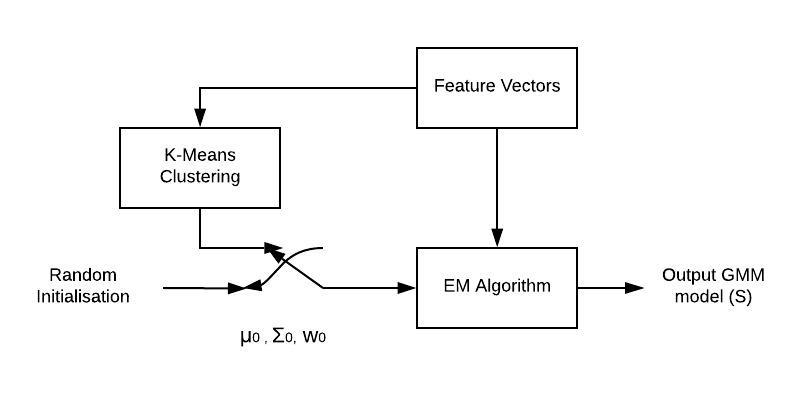
\includegraphics[scale=.65]{Images/gmm_em.jpeg}}
\caption{Basic block diagram of GMM training.}
\label{gem}
\end{figure} 
\subsubsection{Expectation Maximization Algorithm}

We have to maximize the likelihood $L(X|S)$ with respect to the model parameters $S=\{w_{i},\mu_{i},\Sigma_{i}\}$, then the partial derivative with respect to $\mu_{i}$ and $\Sigma_{i}$ can be written as:

\begin{equation}
\begin{aligned}
\label{lpd}
 \frac{\partial L(X|S)}{\partial \mu_{i}}=&\frac{\sum_{j=1}^{T} w_{i}P(x_{j}|\theta_{i})\Big(\frac{x_{j}-\mu_{i}}{\Sigma_{i}}\Big)}{\sum_{i=1}^{M_{g}} w_{i}P(x_{j}|\theta_{i})}\\
 \frac{\partial L(X|S)}{\partial \Sigma_{i}}=&\frac{\sum_{j=1}^{T} w_{i}P(x_{j}|\theta_{i})\Big(\frac{\Sigma_{i}^{-1}(x_{j}-\mu_{i})(x_{j}-\mu_{i})^{T}\Sigma_{i}^{-1}}{2}-\frac{1}{2\Sigma_{i}}\Big)}{\sum_{i=1}^{M_{g}} w_{i}P(x_{j}|\theta_{i})}, \quad i=1,2,\ldots,M_{g}
 \end{aligned}
\end{equation}

Equating the partial derivatives in the equation~\ref{lpd} to zero and by assuming,
\begin{equation}
\label{gm}
    \gamma_{ij}=\frac{w_{i}P(x_{j}|\theta_{i})}{{\sum_{i=1}^{M_{g}} w_{i}P(x_{j}|\theta_{i})}}
\end{equation}

the $\mu_{i}$ and $\Sigma_{i}$ can be written as:

\begin{equation}
\begin{aligned}
\label{opmv}
\mu_{i}=&\frac{\sum_{j=1}^{T}\gamma_{ij}x_{j}}{\sum_{j=1}^{T}\gamma_{ij}}\\
\Sigma_{i}=&\frac{\sum_{j=1}^{T}\gamma_{ij}(x_{j}-\mu_{i})(x_{j}-\mu_{i})^{T}}{\sum_{j=1}^{T}\gamma_{ij}}, \quad i=1,2,\ldots,M_{g}
\end{aligned}
\end{equation}

%
There is a constraint of $\sum_{i=1}^{M_{g}}w_{i}=1$, so to find the optimal value, we have to use Lagrange constraint optimization, the modified objective function can be written as:
\begin{equation}
\label{obj}
    \max_{w_{i}} \quad L(X|S)+\eta \Bigg(\sum_{i=1}^{M_{g}}w_{i}-1 \Bigg)
\end{equation}

The partial derivative of equation~\ref{obj} with respect to $w_{i}$ can be written as:
\begin{equation}
\begin{aligned}
\label{wop}
\frac{\partial \Bigg(L(X|S)+\eta \Bigg(\sum_{i=1}^{M_{g}}w_{i}-1 \Bigg)\Bigg)}{\partial w_{i}}=&\sum_{j=1}^{T}\frac{P(x_{j}|\theta_{i})}{\sum_{i=1}^{M_{g}} w_{i}P(x_{j}|\theta_{i})}\\
 =&\sum_{j=1}^{T} \frac{\gamma_{ij}}{w_{i}}+\eta\\
\end{aligned}
\end{equation}
Equating the partial derivatives in the equation~\ref{wop} to zero, 

\begin{equation}
\label{lsl}
    \begin{aligned}
     \sum_{j=1}^{T}\gamma_{ij}=&-\eta(w_{i})\\
     -\eta (w_{1}+w_{2}+\ldots+w_{M_{g}})=&\sum_{i=1}^{M_{g}}\sum_{j=1}^{T}\gamma_{ij}\\
    - \sum_{i=1}^{M_{g}}\sum_{j=1}^{T}\gamma_{ij}=&\eta \quad \quad  \Bigg(as \quad \sum_{i=1}^{M_{g}}w_{i}=1\Bigg)
    \end{aligned}
\end{equation}

From the definition of $\gamma_{ij}$ (as per equation~\ref{gm}) we can say, $\gamma_{ij}$ is the probability of $j^{th}$ vector corresponds to $i^{th}$ Gaussian. So, $\sum_{i=1}^{M_{g}}\gamma_{ij}=1$, and $\sum_{j=1}^{T}\sum_{i=1}^{M_{g}}\gamma_{ij}=T$.

From equation~\ref{lsl}, we get $\eta = -T$, and $w_{i}$ can be written as:
\begin{equation}
w_{i}=\frac{1}{T}\sum_{j=1}^{T}\gamma_{ij}
\end{equation}

Putting all together, we can write the estimated values of $w_{i},\mu_{i}$, and $\Sigma_{i}$ as:
\begin{equation}
\begin{aligned}
\label{op}
\mu_{i}=&\frac{\sum_{j=1}^{T}\gamma_{ij}x_{j}}{\sum_{j=1}^{T}\gamma_{ij}}\\
\Sigma_{i}=&\frac{\sum_{j=1}^{T}\gamma_{ij}(x_{j}-\mu_{i})(x_{j}-\mu_{i})^{T}}{\sum_{j=1}^{T}\gamma_{ij}}\\
w_{i}=&\frac{1}{T}\sum_{j=1}^{T}\gamma_{ij}, \quad i=1,2,\ldots,M_{g}\\
where, \quad \gamma_{ij}=&\frac{w_{i}P(x_{j}|\theta_{i})}{{\sum_{i=1}^{M_{g}} w_{i}P(x_{j}|\theta_{i})}}
\end{aligned}
\end{equation}
From the above equation~\ref{op}, It is worth to note that the results don't constitute a close form solution. The parameters of the GMM depends on $\gamma_{ij}$ value, which again depends on the model parameters. This suggests, solve for a analytic solution is not possible. The solution can be obtain by using a simple iterative procedure. Which is well known as EM algorithm. We first choose some initial values for the means, covariances, and weights. Then by considering the initial values, the $\gamma_{ij}$ value is computed (known as expectation step) and then using the $\gamma_{ij}$ value the means, covariances, and weights values are computed (known as maximization step). The equation~\ref{op} can be modified as:

\begin{equation}
\begin{aligned}
\label{opi}
\gamma_{ij}^{k+1}=&\frac{w_{i}^{k}P(x_{j}|\theta_{i}^{k})}{{\sum_{i=1}^{M_{g}} w_{i}^{k}P(x_{j}|\theta_{i}^{k})}}\\
\mu_{i}^{k+1}=&\frac{\sum_{j=1}^{T}\gamma_{ij}^{k+1}x_{j}}{\sum_{j=1}^{T}\gamma_{ij}^{k+1}}\\
\Sigma_{i}^{k+1}=&\frac{\sum_{j=1}^{T}\gamma_{ij}^{k+1}(x_{j}-\mu_{i}^{k+1})(x_{j}-\mu_{i}^{k+1})^{T}}{\sum_{j=1}^{T}\gamma_{ij}^{k+1}}\\
w_{i}^{k+1}=&\frac{1}{T}\sum_{j=1}^{T}\gamma_{ij}^{k+1}, \quad i=1,2,\ldots,M_{g}\\
\end{aligned}
\end{equation}

The process continues until $L(X|S^{k+1}) \geq L(X|S^{k})$. In general the EM algorithm takes many more iteration for convergence, thus K-means algorithm is used to initialize the model parameters. For each observation X, if the $\gamma_{ij}$ value is given, than its known as complete data, in such cases the analytic solution can be obtained using equation~\ref{op}. But, in practice only observations are given known as incomplete data. In such situation, EM algorithm is used to estimate the model parameters.  
\subsubsection{Maximum a posteriori (MAP) Parameter estimation}
\label{secmap}
The parameters of the GMM can also be estimated using MAP estimation. This approach is generally used in the pattern recognition tasks where the available labeled training data is limited. In speaker and language recognition task this approach is used to derive the adapted speaker/language model by adapting the training vectors with the universal background model (UBM)~\cite{reynolds2000speaker}. 

Like EM algorithm, the MAP estimation is also a two step process.
\begin{enumerate}
    \item Step 1: The sufficient statistics of the training data are computed for each mixture in the prior model (The model computed using ML estimation).
    \item Step 2: The new estimated sufficient statistics are combined with the old sufficient statistics sufficient statistics from the prior mixture parameters using a data-dependent mixing coefficient. 
\end{enumerate}
The data-dependent mixing coefficient is designed so that mixtures with high counts of new data rely more on the new sufficient for final parameter estimation and mixtures with low counts of new data rely more on the old sufficient statistics for final parameter estimation. The prior model is a large GMM (known as UBM) that is trained using ML estimation with large amount of data which encompasses the different kinds of speech that may be encountered by the system during training. These different kinds may include different channel conditions, composition of speakers/languages, acoustic conditions, etc.

Given a prior model ($S^{prior}$) and training vectors from the desired class ($X=\{x_{1},x_{2},\ldots,x_{T}\}$), the sufficient statistics with respect to the prior model can be computed using equation~\ref{s1map}.

\begin{equation}
\label{s1map}
    \begin{aligned}
     \gamma_{ij}=&\frac{w_{i}^{prior}P(x_{j}|\theta_{i}^{prior})}{\sum_{i=1}^{M_{g}}w_{i}^{prior}P(x_{j}|\theta_{i}^{prior})}\\
     n_{i}=&\sum_{j=1}^{T}\gamma_{ij}\\
     E_{i}(X)=&\frac{1}{n_{i}}\sum_{j=1}^{T}\gamma_{ij}x_{j}\\
     E_{i}(X^{2})=&\frac{1}{n_{i}}\sum_{j=1}^{T}\gamma_{ij}~\mbox{Diag}(x_{j}x_{j}^{T})
    \end{aligned}
\end{equation}

The new sufficient statistics computed from the training data then used to update the prior sufficient statistics for mixture $i$ to create the adapted parameters for mixture $i$ by using the equation~\ref{s2map} 
\begin{equation}
\label{s2map}
    \begin{aligned}
     \hat{w_{i}}=&\Bigg[\frac{\alpha_{i}^{w}n_{i}}{T}+(1-\alpha_{i}^{w})w_{i}\Bigg]\Gamma\\
     \hat{\mu_{i}}=&\alpha_{i}^{m}E_{i}(x_{t})+(1-\alpha_{i}^{m})\mu_{i}\\
      \hat{\Sigma_{i}}=&\alpha_{i}^{v}E_{i}(x_{t}^{2})+(1-\alpha_{i}^{v})(\mbox{Diag}~( \Sigma_{i})+\mu_{i}^{2})-\hat{\mu_{i}}^{2}
    \end{aligned}
\end{equation}
 A scale factor $\Gamma$ is used, which ensures that all the new mixture weights sum to 1. $\alpha_{i}^{w},\alpha_{i}^{m}$ and $\alpha_{i}^{v}$ are the adaptation coefficient which controls the balance between the old and new model parameter estimates. $\alpha_{i}$ is defined as:
 \begin{equation}
   \alpha_{i}^{w}=\alpha_{i}^{m}= \alpha_{i}^{v}=\alpha_{i}=\frac{n_{i}}{n_{i}+r}
 \end{equation} 
 \begin{figure}[h]
\centering{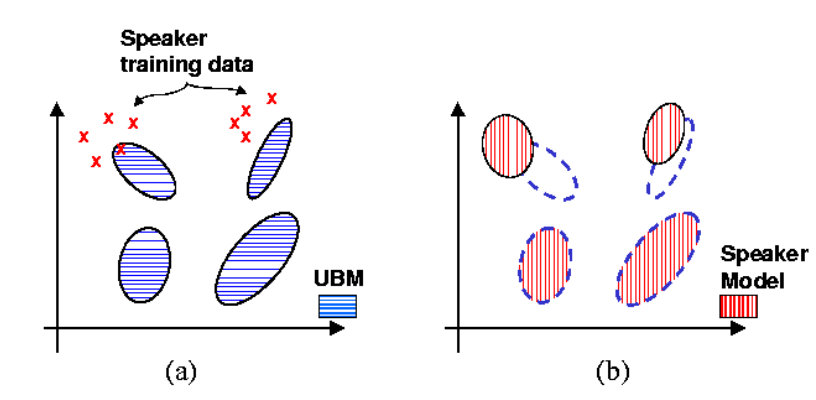
\includegraphics[scale=.45]{Images/MAP.png}}
\caption{(a) The training vectors (x’s) are probabilistically mapped
into the UBM (prior) mixtures. (b) The adapted mixture parameters are derived using the statistics of the new data and the UBM (prior) mixture parameters. The adaptation is data dependent, so UBM (prior) mixture parameters are adapted by different amounts~\cite{reynolds1995speaker}.}
\label{map}
\end{figure}
 where r is a fixed relevance factor, which determines the extent of mixing of the old and new estimates of the parameters. If a mixture component has a low probabilistic count ($n_{i}$) of new data, then $\alpha_{i}\Rightarrow 0$ causing the de-emphasis of the new (potentially under-trained) parameters and the emphasis of the old (better trained) parameters. For mixture components with high probabilistic counts, $\alpha_{i}\Rightarrow 1$ causing the use of the new class-dependent parameters. The pictorial representation of the same is presented in figure~\ref{map}. The relevance factor is a way of controlling how much new data should be observed in a mixture before the new parameters begin replacing the old parameters. Thus, this approach is robust to limited training data.
 

 \subsection{Testing of GMMs}
\begin{figure}[h]
\centering{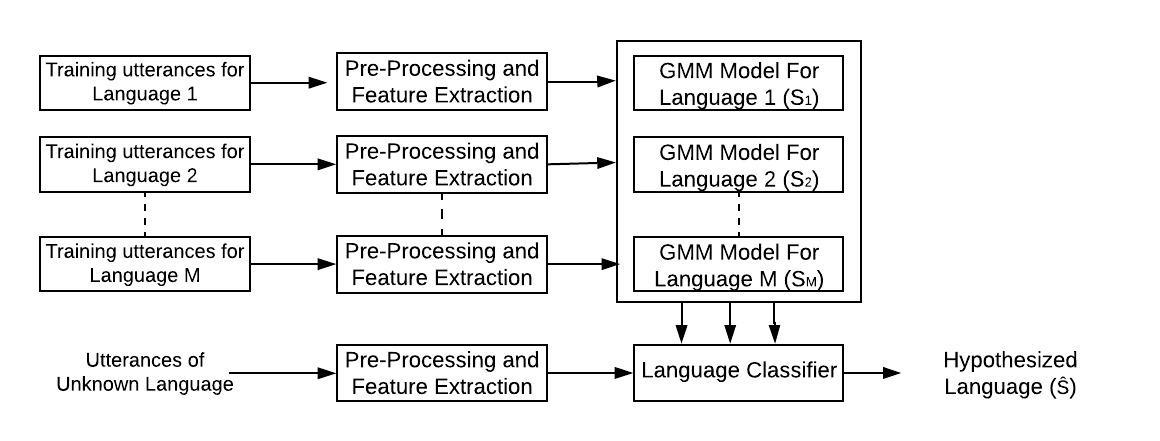
\includegraphics[scale=.65]{Images/gmm.jpeg}}
\caption{Basic block diagram of language identification using GMM.}
\label{gmm}
\end{figure} 

 In the testing phase the objective is to identify the hypothesized model from a set of models $\{S_{1}, S_{2},...,S_{M}\}$ given a set of testing vectors $X=\{x_{1}, x_{2},.., x_{T}\}$. The identified model ($\hat{S}$) can be evaluated using equation~\ref{tllk}. 

\begin{equation} 
\begin{aligned}
\label{tllk}
\hat{S} =&\mbox{arg}~\max_{1 \leq i \leq M} P(S_{i}|X)\\
        =&\mbox{arg}~\max_{1 \leq i \leq M} \frac{P(X|S_{i})}{P(X)}P(S_{i})
\end{aligned}
\end{equation}
 Using ML detection criteria (i.e Assuming equal probability occurrence of all the models )  and the statistical independence of the testing vectors, the decision rule for the most probable model can be redefined as:
 \begin{equation}
  \hat{S}=\mbox{arg}~\max_{1 \leq i \leq M}\sum_{j=1}^{T}~\mbox{log}(P(x_{j}|S_{i}))
 \end{equation} 

The basic block diagram of Language identification task using GMM based training and testing are presented in figure~\ref{gmm}. 

\section{Gaussian Mixture Model and Universal Background Model (GMM-UBM)}
\label{cgmmubm}

The GMM-UBM approach is a vary successful technique for speaker recognition applications. Later by inspiring from the performance of GMM-UBM based speaker recognition systems, people start using GMM-UBM technique in language identification task. After GMM-UBM technique dominantly used in language identification task.
\begin{figure}[h]
\centering{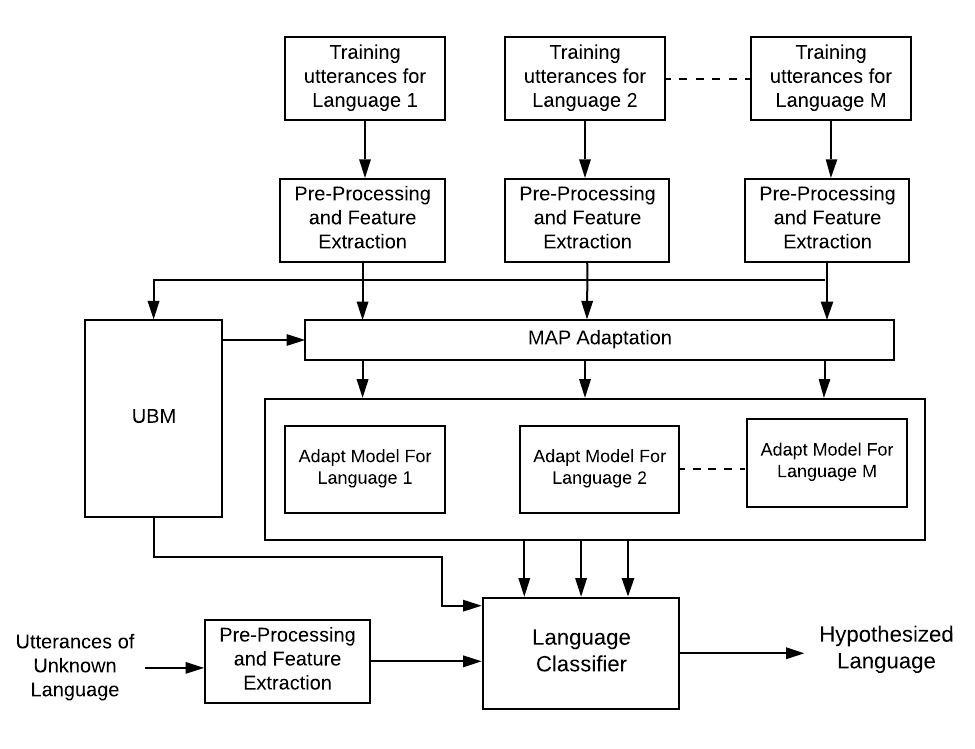
\includegraphics[scale=.65]{Images/ubm.jpeg}}
\caption{Basic block diagram of language identification using GMM-UBM.}
\label{ubm}
\end{figure}

The basic block diagram of GMM-UBM based language identification system is shown in figure~\ref{ubm}. The training phase of GMM-UBM technique is divided into two distinct stages. First a set of feature vector from a number of different languages (typically data from all possible languages used for testing) are taken to train a single GMM (known as UBM). The UBM is considered to represent the characteristics of all different languages. In the second stage the UBM is adapted for each of the languages in the system using MAP adaptation. The detail of MAP adaptation training procedure is described in section~\ref{secmap}. The idea behind MAP adaptation is that, the parameters of the Gaussian which show higher probability towards the language training data will tends towards the parameters of the training data, and the parameters of the mixture show lower probability to the language training data will remain fairly close to the original UBM. The MAP adaptation of the GMM parameters is often applied to the means of the mixture components rather than means, variances and weights (i.e. $\alpha^{v},\alpha^{w}=0$)~\cite{ambikairajah2011language}.      

In the testing phase, given a set of testing vectors $\{x_{1},x_{2},\ldots,x_{T}\}$ , UBM model $S^{ubm}$ and the adapt models of each language $\{S_{i}^{adapt}\}_{i=1}^{M}$, the identified language model can be evaluated using equation~\ref{gmmubmeva}. Where $M$ is the total no of languages used in the system.

\begin{equation}
    \label{gmmubmeva}
   \hat{S}=\mbox{arg}~\max_{1 \leq i \leq M}\sum_{j=1}^{T}\bigg[~\mbox{log}(P(x_{j}|S_{i}^{adapt})) - ~\mbox{log}(P(x_{j}|S^{ubm})\bigg]
\end{equation}

\section{I-vector based language identification system}
\label{ivector}
Language recognition and speaker recognition has many similarities in terms of technical formulation. Thus, in literature most of the descriptors and modeling techniques used to perform language identification task are borrowed from speaker recognition. In case of speaker recognition, in GMM-UBM based statistical modeling, the MAP adaptation not only adapt the speaker specific information but also adapts the channel and session variations. Thus to improve the speaker recognition performance, needs a modeling technique which can model the speaker specific information and other variability separately or to model all the information, suppress the other variability and retain the speaker specific information. In~\cite{kenny2005joint}, the authors propose a method to model all the variations separately. They represented a speaker utterance by a supervector (M), that consists of additive components of speaker and channel/session subspace. This technique is well known as joint factor analysis (JFA).  The speaker dependent supervector is defined as:
\begin{equation}
    \label{jfa}
    M=m+Vy+Ux+Dz
\end{equation}
where m is a speaker and session independent supervector (generally mean vector of UBM having $M_{g}D\times 1$ dimension). $V$ and $D$ define a speaker subspace (eigenvoice matrix and diagonal residual respectively), and $U$ defines a session or channel subspace (eigen channel matrix). The vector $y$, $z$ and $x$ are the speaker and channel/session dependent factors in their respective subspace and each is assumed to be a random variable with a standard normal distribution ($N(0,I)$). In JFA, first the subspaces (i.e $V$, $D$ and $U$) have to be estimated from the appropriate labeled corpora, than the speaker and session factors (i.e $y$, $z$ and $x$) have to be computed for the target utterances. The scoring is done by computing the likelihood of the test utterance vectors against the session compensated speaker model ($M-Ux$). In~\cite{dehak2011front}, the authors slightly modify the modeling technique to reduce the computation and enhance the recognition performance. The authors proposed a single subspace modeling instead of two subspace (speaker and channel separately). This single subspace is known as total variability subspace. The total variability subspace contains both the speaker and channel variability information. The new speaker and channel dependent supervector can be  defined as:
\begin{equation}
    \label{ivec}
    M=m+Tw
\end{equation}
where $T$ is the total variability subspace and $w$ is the speaker and channel dependent vector (known as identity vector/ i-vector). $T$ is a rectangular matrix of low rank and $w$ is a vector having standard normal distribution. After i-vector extraction some channel compensation techniques (like linear discriminative analysis (LDA), within class covariance normalization (WCCN) and nuisance attribute projection (NCA)) are used to suppress the channel variability. A cosine kernel scoring technique is used to find the recognition performance. The block diagram of i-vector based language recognition system is shown in figure ~\ref{i-vec}. 

\begin{figure}[h]
\centering{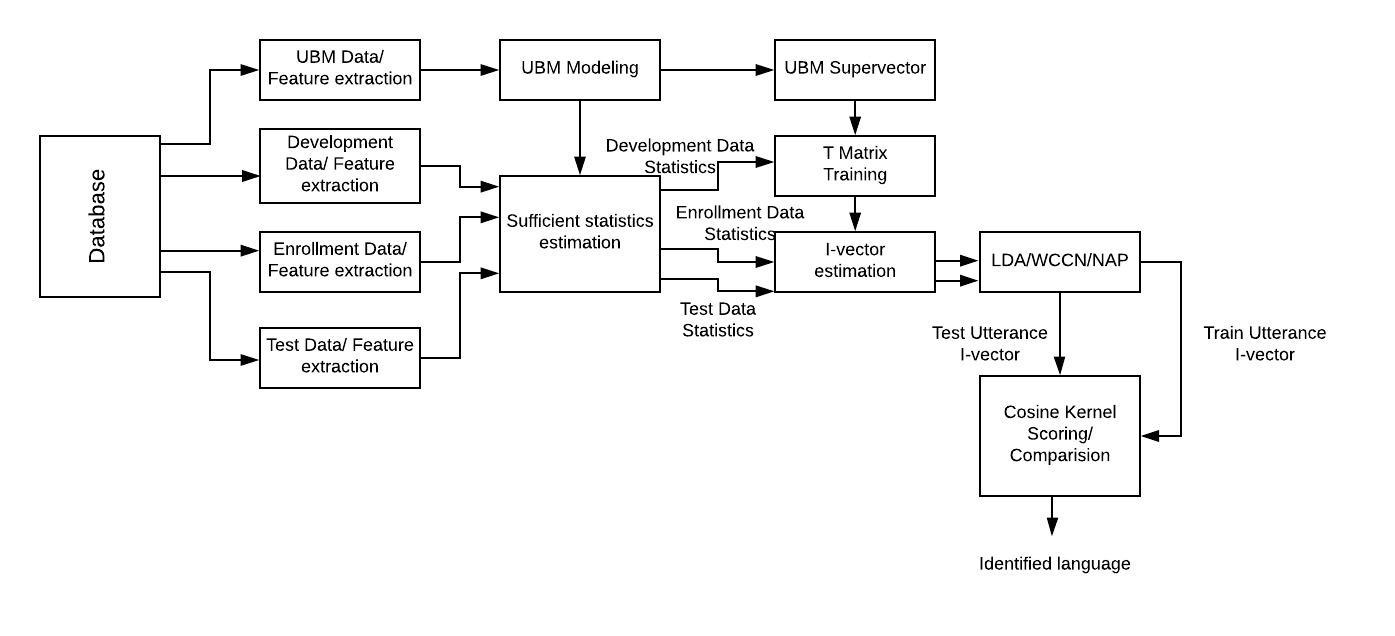
\includegraphics[scale=.65]{Images/i_vector.jpeg}}
\caption{Basic block diagram of language identification using i-vector.}
\label{i-vec}
\end{figure}
From the figure~\ref{i-vec}, it has been seen that, the whole dataset is segmented into four parts: UBM data, development data, enrollment data, test data. UBM data consists of data of all the languages, used to build UBM models as described in section~\ref{cgmmubm}. The development data segment also consists of utterances from all the languages, used to estimate the total variability matrix. After the estimation of total variability matrix (T matrix), the hidden variable $w$, known as i-vector is estimated from each utterance of the enrollment and test data. The i-vector $w$, which can be defined by its posterior distribution conditioned to the Baum-Welch statistics for a given utterance. The posterior distribution is a Gaussian distribution and the Baum-Welch sufficient statistics will be estimated from the UBM. Suppose we have $T$ frames $\{x_{1}, x_{2}, \ldots, x_{T}\}$ of an utterance and the UBM composed of $M_{g}$ mixture components defined in some feature space of dimension $D$. The Sufficient statistics for a given utterance is given by:
\begin{equation}
    \begin{aligned}
     N_{i}=&\sum_{j=1}^{T}\gamma_{ij} \quad (zeroth ~order ~statistics)\\
     F_{i}=&\sum_{j=1}^{T}\gamma_{ij}x_{j} \quad (first ~order ~statistics)\\
     S_{i}=&\mbox{diag}\Bigg[\sum_{j=1}^{T}\gamma_{ij}x_{j}x_{j}^{*}\Bigg], \quad i=1,2,\ldots,M_{g} \quad (second ~order ~statistics)
    \end{aligned}
\end{equation}
where $x_{j}^{*}$ is the Hermitian transpose of vector $x_{j}$ and $\gamma_{ij}=\frac{w_{i}P(x_{j}|\theta_{i})}{{\sum_{i=1}^{M_{g}} w_{i}P(x_{j}|\theta_{i})}}$ (from equation~\ref{gm}).  In order to estimate the i-vector, we need to centralize the first and second order sufficient statistics. The centralized statistics is given by:
\begin{equation}
    \begin{aligned}
     \tilde{F}_{i}=&\sum_{j=1}^{T}\gamma_{ij}(x_{j}-m_{i}) \\
        =&\sum_{j=1}^{T}\gamma_{ij}x_{j}-\sum_{j=1}^{T}\gamma_{ij}m_{i}\\
        =&F_{i} - N_{i}m_{i}\\
     \tilde{S_{i}}=&\mbox{diag}\Bigg[\sum_{j=1}^{T}\gamma_{ij}(x_{j}-m_{i})(x_{j}-m_{i})^{*}\Bigg], \quad i=1,2,\ldots,M_{g}\\
     =& S_{i}-\mbox{diag}(F_{i}m_{i}^{*}+m_{i}F_{i}^{*}-N_{i}m_{i}m_{i}^{*})
    \end{aligned}
\end{equation}
where $m_{i}$ is the mean vector of the $i^{th}$ mixture. We can write the statistics in the matrix format as:
\begin{equation}
    \begin{aligned}
     N_{m}=&\begin{bmatrix} 
        N_{1}*I &     &                 \\
                &\ddots&                \\
                &       & N_{M_{g}}*I 
        \end{bmatrix}\\
    F_{m}=&\begin{bmatrix}
            \tilde{F}_{1}\\
            \vdots      \\
            \tilde{F}_{M_{g}}
            \end{bmatrix}\\
    S_{m}=&\begin{bmatrix} 
        \tilde{S}_{1} &     &                 \\
                &\ddots&                \\
                &       & \tilde{S}_{M_{g}} 
        \end{bmatrix}\\        
    \end{aligned}
\end{equation}
where $N_{m}$ is a matrix of dimension $M_{g}D \times M_{g}D$, $I$ is a identity matrix of dimension $D \times D$, $F_{m}$ is a  vector of dimension $M_{g}D \times 1$ and $S_{m}$ is a matrix of dimension $M_{g}D \times M_{g}D$. In~\cite{kenny2005joint} from Theorem 2 we can write the distribution of the hidden variable (w) is $N(L_{T}^{-1}*T^{*}*\Sigma^{-1}*F_{m},L_{T}^{-1})$. The i-vector can be computed as $E(w)=L_{T}^{-1}*T^{*}*\Sigma^{-1}*F_{m}$. where $E(w)$ is the expectation of vector $w$, $\Sigma$ is the variance of the UBM, $L_{T}= I+T^{*}\Sigma^{-1}N_{m}T$ and $T$ is the total variability matrix.

\subsection{T Matrix training}
\begin{enumerate}
    \item Step 1: Initialize the T matrix randomly having dimension $M_{g}D \times Dimension~of~i-vector$
    \item Step 2: Compute: $L_{T}=I+T^{*}\Sigma^{-1}*N_{m}*T$
    \item Step 3: Accumulate the statistics across utterances:
    \begin{equation}
        \begin{aligned}
         ^{a}N_{i}=&\sum_{u}N_{i}(u)\\
         ^{a}A_{i}=&\sum_{u}N_{i}(u)L_{T}^{-1}\\
         ^{a}C=&\sum_{u}F_{m}(u)(L_{T}^{-1}(u)*T^{*}*\Sigma^{-1}*F_{m}(u))\\
         ^{a}N_{m}=&\sum_{u}N_{m}(u)
        \end{aligned}
    \end{equation}

    \item Step 4: Compute T matrix:
    \begin{equation}
        T=\begin{bmatrix}
        T_{1}\\
        \vdots\\
        T_{M_{g}}
        \end{bmatrix}=\begin{bmatrix}
        A_{1}^{-1}*C_{1}\\
        \vdots\\
        A_{M_{g}^{-1}*C_{M_{g}}}
        \end{bmatrix}, \quad where \quad C=\begin{bmatrix}
        C_{1}\\
        \vdots\\
        C_{M_{g}}
        \end{bmatrix}
    \end{equation}
    \item Step 5: Compute covariance update (optional):
    \begin{equation}
        \Sigma= (^{a}N_{m})^{-1}\Bigg[\sum_{u}S_{m}(u)-\mbox{diag}(C*T^{*})\Bigg]
    \end{equation}
    \item Step 6: Iterate step 2 to step 4 (or step 5) approximately 20 times to get the estimate of the T matrix.
\end{enumerate}
In the literature, people have not used the second order statistics($S_{m}$) for speaker and language recognition task, in such cases step 5 is not required.
 \subsection{I-vector estimation}
 After the estimation of T matrix the i-vectors from each utterances of the enrollment set and test set is computed using equation~\ref{eivec}.
 \begin{equation}
 \label{eivec}
    w(u)= L_{T}^{-1}(u)*T^{*}*\Sigma^{-1}*F_{m}(u)
 \end{equation}
 
 \subsection{Cosine kernel scoring}
 Cosine kernel scoring is technique to find the cosine kernel between the train language i-vectors and test i-vector. Suppose there are L languages having each $K_{1},K_{2}, \ldots, K_{L}$ utterances and lets denote the train language i-vector as $w_{lk}$ and the test utterance i-vector as $w_{test}$. The identified language ($\hat{S}$) can be written as
 
 \begin{equation}
     \hat{S}=\mbox{arg}~\max_{1 \leq l \leq L} \sum_{k=1}^{K_{l}} Score_{lk}=\mbox{arg}~\max_{1 \leq l \leq L} \sum_{k=1}^{K_{l}} \frac{<w_{lk},w_{test}>}{||w_{lk}||||w_{test}||}
 \end{equation}
 
 \subsection{Intersession compensation techniques}
 \label{lda}
 The intersession compensation techniques are used to enhance the inter-class variations and to suppress the intra-class variations.  Generally there are three dominantly used intersession compensation technique to enhance the recognition performance, while the classes are modeled in total variability space. These three techniques are: linear discriminant analysis (LDA), within class covariance normalization (WCCN), nuisance attribute projection (NAP). 
 \subsubsection{Linear discriminant analysis (LDA)}
 LDA is a technique of dimensionality reduction, widely used in the task of pattern recognition. The motivation of using LDA in i-vector based language recognition task is that, as all the utterances of a given language are assume to represent one class, LDA attempts to define new special axes that minimize the intra-class variance caused by channel and speaker effects, and to maximize the variance between languages. This approach searches a new orthogonal axes to better discriminate between classes. The LDA optimization problem can be defined according to the ratio given in equation~\ref{ld1}. 
 \begin{equation}
     \label{ld1}
     J(v)=\frac{v^{t}S_{b}v}{v^{t}S_{w}v}
 \end{equation}
 The ratio is often referred as the Rayleigh coefficient for space direction $v$. $S_{b}$ and $S_{w}$ are the between class and the within-class variance between matrix and are calculated as follows:
 \begin{equation}
 \begin{aligned}
   S_{b}=&\sum_{l=1}^{L}(w_{l}-\bar{w})(w_{l}-\bar{w})^{t}\\
   S_{w}=&\sum_{l=1}^{L}\frac{1}{K_{L}}\sum_{k=1}^{K_{L}}(w_{k}^{l}-\bar{w}_{l})(w_{k}^{l}-\bar{w}_{l})^{t}
 \end{aligned}
 \end{equation}
 where $\bar{w}_{l}=\frac{1}{K_{L}}\sum_{k=1}^{K_{L}}w_{k}^{l}$ is the mean of i-vectors for each language. $\bar{w}$ is the mean of i-vector for all the utterances. The maximization is used to define a projection matrix A composed by the best eigen vectors (those with highest eigen values) of the general eigen value equation:
 \begin{equation}
     \begin{aligned}
      S_{b}v=&\lambda S_{w}v\\
      S_{b}S_{w}^{-1}v=&\lambda v
     \end{aligned}
 \end{equation}
 where $\lambda$ is the diagonal matrix of eigenvalues. The the projection matrix is obtained by taking the eigen vectors of the larger eigenvalues (i.e $A=V(:,1:no~of~top~eigen~values)$).The identified language ($\hat{S}$) can be written as:
 
 \begin{equation}
     \hat{S}=\mbox{arg}~\max_{1 \leq l \leq L} \sum_{k=1}^{K_{l}} Score_{lk}=\mbox{arg}~\max_{1 \leq l \leq L} \sum_{k=1}^{K_{l}} \frac{<A^{t}w_{lk},A^{t}w_{test}>}{||A^{t}w_{lk}||||A^{t}w_{test}||}
 \end{equation}
  
  \subsubsection{Within class covariance normalization (WCCN)}
  This technique was first introduced in~\cite{hatch2006within}. In the study, they applied this approach in SVM modeling based on linear separation between target speaker and imposter using one verses all decision. WCCN techniques uses inverse of within-class covariance to normalize the cosine kernel. The resulting solution by a generalized linear kernel form can be written as given in ~\cite{hatch2006within}:
  \begin{equation}
      k(w_{1},w_{2})=w_{1}^{t}Rw_{2}
  \end{equation}
  where $R$ is a symmetric positive semi-definite matrix. The optimal normalized kernel matrix is given by $R=W^{-1}$. W is a within class covariance matrix, calculated as:
  \begin{equation}
      W=\frac{1}{L}\sum_{l=1}^{L}\frac{1}{K_{L}}\sum_{k=1}^{K_{L}}(w_{k}^{l}-\bar{w}_{l})(w_{k}^{l}-\bar{w}_{l})^{t}
  \end{equation}
  In order to preserve the inner product form of the cosine kernel, a feature-mapping function $\varphi$ can be defined as:
  \begin{equation}
      \varphi(w)=B^{t}w
  \end{equation}
  where B is obtained through Cholesky decomposition of matrix $W^{-1}=BB^{t}$. The WCCN algorithm uses the within-class covariance matrix to normalize the cosine kernel function to normalize the cosine kernel functions in order to compensate for intersession variability, while guaranteeing conservation of directions in space. The identified language ($\hat{S}$) can be written as:
 
 \begin{equation}
     \hat{S}=\mbox{arg}~\max_{1 \leq l \leq L} \sum_{k=1}^{K_{l}} Score_{lk}=\mbox{arg}~\max_{1 \leq l \leq L} \sum_{k=1}^{K_{l}} \frac{<B^{t}w_{lk},B^{t}w_{test}>}{||B^{t}w_{lk}||||B^{t}w_{test}||}
 \end{equation} 
 
 \subsubsection{Nuisance attribute projection (NAP)}
 The nuisance attribute projection algorithm is presented in~\cite{campbell2006svm}. It is based on finding an appropriate projection matrix intended to remove the nuisance direction. The projection matrix carries out an orthogonal projection in channel's and speaker's complimentary space, which depends only on language class information. The projection matrix is formulated as:
 \begin{equation}
     P=I-RR^{t}
 \end{equation}
 where $R$ is a rectangular matrix of low rank, whose columns are the eigen vectors ($Wr=\lambda r$) having the best eigen values of the within-class covariance matrix (W) computed as:
  \begin{equation}
      W=\frac{1}{L}\sum_{l=1}^{L}\frac{1}{K_{L}}\sum_{k=1}^{K_{L}}(w_{k}^{l}-\bar{w}_{l})(w_{k}^{l}-\bar{w}_{l})^{t}
  \end{equation}
   
 The identified language ($\hat{S}$) using NAP can be written as:
 
 \begin{equation}
     \hat{S}=\mbox{arg}~\max_{1 \leq l \leq L} \sum_{k=1}^{K_{l}} Score_{lk}=\mbox{arg}~\max_{1 \leq l \leq L} \sum_{k=1}^{K_{l}} \frac{<P^{t}w_{lk},P^{t}w_{test}>}{||P^{t}w_{lk}||||P^{t}w_{test}||}
 \end{equation} 



\section{Feedforward network based model}
\label{ffnn}
\begin{figure}[h]
\centering{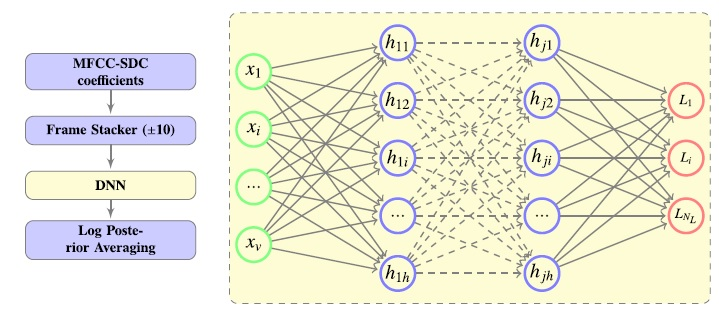
\includegraphics[scale=.65]{Images/ffn.jpg}}
\caption{Feedforward network based classifier~\cite{lopez2016use}.}
\label{ffn}
\end{figure}

The impressive gain in performance obtained using deep neural networks (DNNs) for automatic speech recognition (ASR) have motivated the application of DNNs in other speech technologies such as language recognition and speaker recognition. Feedforward neural network is a fully connected network, which shows the direct use of DNN in the recognition task. In this approach, a fully connected network with multiple hidden layers is trained using back-propagation algorithm to perform recognition task. The output layer of this network has the number of neurons (nodes) same as the number of classes in the recognition task, whereas the input layer has the number of nodes same as the dimension of input feature vector (refer figure~\ref{ffn}). In general, the MFCC/SDC features are computed and then stacked with the feature vectors of the neighboring frames and then given input to the network.  After training is over, testing is performed using the feature vectors of the speech utterances.  For a test utterance, the output score is computed as:
\begin{equation}
    score_{l}=\frac{1}{N}\sum_{t=1}^{N}log p(L_{l}|x_{t},\Theta)
\end{equation}
where $p(L_{l}|x_{t},\Theta)$ represents the class probability output for language l corresponding to the input example at time $t$, $x_{t}$ is the feature vector and $\Theta$ is the parameter of the DNN.

For a test utterance, the output node giving the highest score is termed as the recognition class.  





\section{Bottleneck feature I-vector model}
DNN architectures can be used for feature extraction. From the human language recognition ability, it has been seen that both acoustic phonetic and phonotactic information are used for recognition. Thus people try to extract the features, which have both the information. This type of feature can be extracted by training a DNN, by providing the feature vector to the input and its corresponding posterior senone probabilities (computed from a DNN based ASR system) to the output of the DNN. After the network is trained, activation value of a hidden layer near to output layer can be taken as a feature vector (known as bottleneck feature (BNF)) by providing acoustic feature vectors as input(refer figure~\ref{bnf}). After the BNF feature is extracted, I-vector framework is used to identify the language( refer to figure~\ref{bnf1}).  
\begin{figure}[h]
\centering{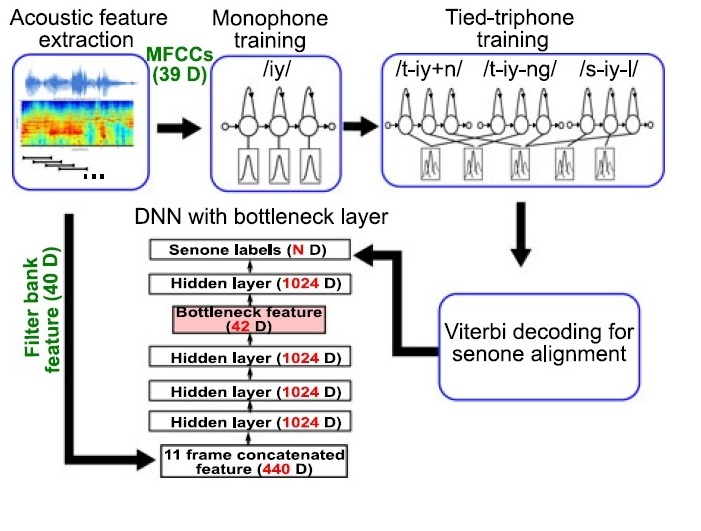
\includegraphics[scale=.30]{Images/dnn_i_vector1.jpg}}
\caption{Bottleneck feature extraction~\cite{zhang2018language}.}
\label{bnf}
\end{figure}
\begin{figure}[h]
\centering{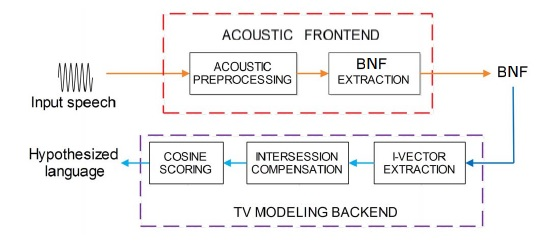
\includegraphics[scale=.60]{Images/bnf.jpg}}
\caption{Bottleneck feature-I-vector based language identification system~\cite{jiang2014deep}.}
\label{bnf1}
\end{figure}

\section{X-vector based modeling}
\label{xvector}
In this approach, the X-vectors are extracted from a trained DNN and then used like I-vectors to perform recognition task. The DNN is trained to discriminate between languages/speakers. The X-vector is a fixed dimensional embedding extracted from the variable length utterance, using a trained time delay neural network (TDNN) based DNN. TDNN is a older approach proposed in~\cite{waibel1989phonemetdnn} on 1989. TDNN works like convolutional neural network (CNN) work on the image to capture local information. The disadvantage of TDNN is, it requires a high amount of data and training time. Thus, in this approach, a subsampling method is used on TDNN to reduce the training time and computational complexity. After sub-sampling as the no of parameters to estimate is reduced, so the training data requirement also reduced. The sub-sampling structure of TDNN is presented in figure~\ref{tdnn}. 
 \begin{figure}[h]
\centering{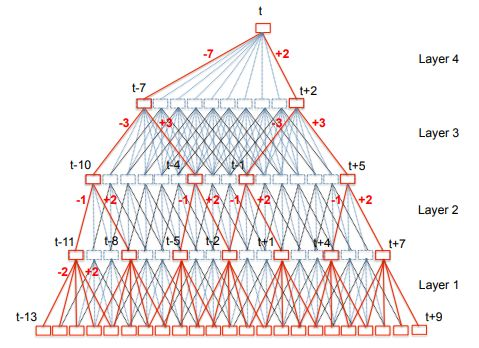
\includegraphics[scale=.62]{Images/tdnn.jpeg}}
\caption{ Computation in TDNN with sub-sampling (red) and
without sub-sampling (blue+red)~\cite{snyder2018spoken}.}
\label{tdnn}
\end{figure}

 \begin{table}
 \caption{The embedding DNN architecture~\cite{snyder2018spoken}.}
 \label{xvac_ar}
\centering\begin{tabular}{|c|c|c|c|}
\hline
Layer                                                   & Layer Context & Total Context & $Input \times Output$ \\ \hline
layer 1                                                 & {[}t-2,t+2{]} & 5             & $5F \times 512 $      \\ \hline
layer 2                                                 & \{t-2,t,t+2\} & 9             & $1536 \times 512$     \\ \hline
layer 3                                                 & \{t-3,t,t+3\} & 15            & $1536 \times 512$     \\ \hline
layer 4                                                 & \{t\}         & 15            & $512 \times 512$      \\ \hline
layer 5                                                 & \{t\}         & 15            & $512 \times 1500$     \\ \hline
\begin{tabular}[c]{@{}c@{}}Stats\\ Pooling\end{tabular} & {[}0,T)       & T             & $1500T \times 3000 $  \\ \hline
Segment 6                                               & \{0\}         & T             & $3000 \times 512 $    \\ \hline
Segment 7                                               & \{0\}         & T             & $512 \times 512$      \\ \hline
Softmax                                                 & \{0\}         & T             & $512 \times L $       \\ \hline
\end{tabular}
\end{table}

The architecture of the sub-sampling based TDNN is given in table~\ref{xvac_ar}. Suppose an input utterance have T feature vectors of F dimension. The input to the network is the concatenation of acoustic features of five frames (2 past, 2 future, 1 current), i.e. a $5*F$ dimension vector. The first five layers operate on speech frames with a small temporal context centered at the current frame t. The statistical pooling layer aggregates all T frame-level outputs from layer 5 and computes it mean and standard deviation (1500 dimension), then concatenate the mean and standard deviation to form 3000 dimension vector (for the whole utterance) and give input to the next layer. The output layer is a softmax layer having the language labels. From segment 6 or segment 7, the embedding vectors are extracted, and then, PLDA and cosine kernel scoring techniques are used to perform language recognition.   
% \section{Language identification, Language verification and Language diarization}
% Like speaker recognition, spoken language recognition can be also be viewed as:
% \begin{itemize}
%     \item Language identification
   
%     \item Language verification
%     \item Language diarization
% \end{itemize}
   
% 
% %\section{Background}
% \lettrine[lines=1]{\textbf{T}}{his} chapter outlines the ..... 
% 
% 
% \section{Section 1}
% "Section Description"
% 
% \section{Section 2}
% "Section Description" \cite{Cite01}, "Section Description"
% \begin{equation}
% \label{eq2}
% x = y + z
% \end{equation}
% 
% Equation \ref{eq1} adds 2 numbers.
% 
% 
% \section{Section 3}
% "Section Description"

\end{spacing} 

\chapter{Delivered System Description }
\chaptermark{ Delivered System Description }
\HRule \\[-0.5cm] % Horizontal line

\label{Chapter1} % For referencing the chapter elsewhere, use \ref{Chapter1}

\lhead{\emph{\textbf{Chapter3:} Delivered System Description }} % This is for the header on each page - perhaps a shortened title

%----------------------------------------------------------------------------------------
%	SECTIONS
%----------------------------------------------------------------------------------------
\section{Database Description}
The whole dataset is subdivided into two parts, i.e. training data and testing data. The training data consists of 11 different language speech data. These languages are American English, CREOL, Cantonese-Chinese, Farsi, Georgian, Korean, Mandarin, Russia, Spanish, Turkey, and Vietnamese. The amount of speech data available in each language is given in table~\ref{Data_amount}. The training data is extracted from multiple corpora, these are OGI-multilingual, NIST 1996, 2003, 2005 LREs, NIST 2004, 2005, 2006, 2008 speaker recognition evaluations (SREs) and NIST 2007 LRE supplementary training data. The test data are extracted from NIST 2009 Evaluation set, which has 3 evaluation conditions, i.e 30 sec, 10 sec and 3 sec.

\begin{table}[ht!]
\centering
\caption{Speech data available in each language}
\label{Data_amount}
\begin{tabular}{|l|l|}
\hline
\textbf{Language name} & \textbf{Approx. duration of speech data} \\ \hline
American English & 26 hours \\ \hline
Creol & 27 hours \\ \hline
Cantonese-Chinese & 26 hours \\ \hline
Farsi & 20 hours \\ \hline
Gorgian & 26 hours \\ \hline
Korean & 10 hours \\ \hline
Mandarin & 15 hours \\ \hline
Russia & 20 hours \\ \hline
Spanish & 14 hours \\ \hline
Turkey & 24 hours \\ \hline
Vietnamese & 18 hours \\ \hline
\end{tabular}
\end{table}
\section{System Description}
\subsection{GMM Based System}
As discussed in section~\ref{gmm_sc} of chapter  1, the same procedure is followed to develop the GMM based system. MATLAB environment is used to develop the system. First, the SDC feature vectors of 56 dimensions (including $C_{0}$, performed CMVN language-wise) each, are extracted from the speech signal, then the GMM of 512 clusters are used to model the feature vectors of each language. The performance obtained using all three testing conditions is tabulated in table ~\ref{gmm_sys}.

\begin{table}[ht!]
\centering
\caption{GMM based system performance}
\label{gmm_sys}
\begin{tabular}{|l|l|l|l|}
\hline
\begin{tabular}[c]{@{}l@{}}Performance \\ Measure\end{tabular} & \multicolumn{1}{c|}{30 sec} & \multicolumn{1}{c|}{10 sec} & \multicolumn{1}{c|}{3 sec} \\ \hline
$EER_{avg}$ & 32.1 & 39.2 & 43.3 \\ \hline
$C_{avg}$ & 30.5 & 37.9 & 42.1 \\ \hline
\begin{tabular}[c]{@{}l@{}}Identification\\ Accuracy\end{tabular} & 56 & 42.1 & 23 \\ \hline
\end{tabular}
\end{table}
\subsection{GMM-UBM Based System}
As discussed in section~\ref{cgmmubm} of chapter  1, the same procedure is followed to develop the GMM-UBM based system. MATLAB environment is used to develop the system. First, the SDC feature vectors of 56 dimensions (including $C_{0}$, performed CMVN language-wise) each, are extracted from the speech signal, then the UBM (cluster size 512) was built using the feature vectors of approx. 2-hour data of each language. Then the training feature vectors of each language were adapted with the UBM to obtain adapt Models for each language. The performance obtained using all three testing conditions is tabulated in table ~\ref{gmm_ubm_sys}.

\begin{table}[ht!]
\centering
\caption{GMM UBM based system performance}
\label{gmm_ubm_sys}
\begin{tabular}{|l|l|l|l|}
\hline
\begin{tabular}[c]{@{}l@{}}Performance \\ Measure\end{tabular} & \multicolumn{1}{c|}{30 sec} & \multicolumn{1}{c|}{10 sec} & \multicolumn{1}{c|}{3 sec} \\ \hline
$EER_{avg}$ & 28.3 & 32.5 & 39.9 \\ \hline
$C_{avg}$ & 27.9 & 32.1 & 38.8 \\ \hline
\begin{tabular}[c]{@{}l@{}}Identification\\ Accuracy\end{tabular} & 64 & 49.1 & 38.1 \\ \hline
\end{tabular}
\end{table}
\subsection{I-vector based System}
As discussed in section~\ref{ivector} of chapter  1, the same procedure is followed to develop the I-vector based system. MATLAB environment is used to develop the system. First, the SDC feature vectors of 56 dimensions (including $C_{0}$, performed CMVN language-wise) each, are extracted from the speech signal, then the UBM (cluster size 512) was built using the feature vectors of approx. 2-hour data of each language. Then all the training feature vectors of each language were used to train the T-matrix, after that 400 dimension I-vectors for each utterance are extracted, LDA and WCCN are used to minimize within-class variance and maximize the between-class variance. The performance obtained using all three testing conditions is tabulated in table ~\ref{ivector_sys}.
\begin{table}[ht!]
\centering
\caption{I-vector based system performance}
\label{ivector_sys}
\begin{tabular}{|l|l|l|l|}
\hline
\begin{tabular}[c]{@{}l@{}}Performance \\ Measure\end{tabular} & \multicolumn{1}{c|}{30 sec} & \multicolumn{1}{c|}{10 sec} & \multicolumn{1}{c|}{3 sec} \\ \hline
$EER_{avg}$ & 24.2 & 29.2 & 33.3 \\ \hline
$C_{avg}$ & 23.9 & 28.9 & 32.6 \\ \hline
\begin{tabular}[c]{@{}l@{}}Identification\\ Accuracy\end{tabular} & 70.1 & 53 & 42 \\ \hline
\end{tabular}
\end{table}
\subsection{Feedforward Network Based System}
As discussed in section~\ref{ffnn} of chapter  1, the same procedure is followed to develop the Feedforward network-based system. Python environment with Keras and TensorFlow libraries was used to develop the system. First, the SDC feature vectors of 56 dimensions (including $C_{0}$, performed CMVN language-wise) each, are extracted from the speech signal, then contexting of previous 10 and future 10 frames were used to provide 1176 dimension input to the neural network. 5 hidden layers with  2048 neurons were used with the Relu activation function. The output layer had 11 neurons with the softmax activation function. The network was trained using stochastic gradient descent with 0.001 learning rate.  The performance obtained using all three testing conditions is tabulated in table ~\ref{ffnn_sys}.
\begin{table}[ht!]
\centering
\caption{Feedforward neural network based system performance}
\label{ffnn_sys}
\begin{tabular}{|l|l|l|l|}
\hline
\begin{tabular}[c]{@{}l@{}}Performance \\ Measure\end{tabular} & \multicolumn{1}{c|}{30 sec} & \multicolumn{1}{c|}{10 sec} & \multicolumn{1}{c|}{3 sec} \\ \hline
$EER_{avg}$ & 25.3 & 30.2 & 36.4 \\ \hline
$C_{avg}$ & 24.8 & 30.09 & 35.9 \\ \hline
\begin{tabular}[c]{@{}l@{}}Identification\\ Accuracy\end{tabular} & 67 & 48 & 39 \\ \hline
\end{tabular}
\end{table}

\subsection{X-vector Based System}
As discussed in section~\ref{xvector} of chapter  1, the same procedure is followed to develop the X-vector based system. Kaldi speaker recognition 2016 recipe was used to develop the system. First, the MFCC feature vectors of 20 dimensions (including $C_{0}$, performed CMVN language-wise) each, are extracted from the speech signal. The architecture given in table~\ref{xvac_ar} of section~\ref{xvector} was used with dropout  of each hidden layer 0,0,0.0001,0.0001,0.0001,0 respectively. The network is trained with 40 epochs. After X-vector is extracted PLDA classifier was used for classification. The performance obtained using all three testing conditions are tabulated in table ~\ref{xvector_sys}.
\begin{table}[ht!]
\centering
\caption{X-vector based system performance}
\label{xvector_sys}
\begin{tabular}{|l|l|l|l|}
\hline
\begin{tabular}[c]{@{}l@{}}Performance \\ Measure\end{tabular} & \multicolumn{1}{c|}{30 sec} & \multicolumn{1}{c|}{10 sec} & \multicolumn{1}{c|}{3 sec} \\ \hline
$EER_{avg}$ & 18.2 & 23.1 & 30.1 \\ \hline
$C_{avg}$ & 17.92 & 22.39 & 29.56 \\ \hline
\begin{tabular}[c]{@{}l@{}}Identification\\ Accuracy\end{tabular} & 79 & 61 & 51 \\ \hline
\end{tabular}
\end{table}
\section{Summary and Discussion}
From the performance of all the systems, it has been observed that the X-vector system outperforms all the other systems. But still, the performance is far from perfect. The performance of the system degrades with the decrease in test utterance duration. Therefore in the future, there is a need for the development of efficient feature extraction and modeling techniques, which will provide a stable Spoken language recognition performance, even if the test duration is small.    
%
\chapter{Introduction}
\chaptermark{ Introduction}
\HRule \\[-0.5cm] % Horizontal line

\label{Chapter1} % For referencing the chapter elsewhere, use \ref{Chapter1}

\lhead{\emph{\textbf{Chapter1:} Introduction}} % This is for the header on each page - perhaps a shortened title

%----------------------------------------------------------------------------------------
%	SECTIONS
%----------------------------------------------------------------------------------------
%
\chapter{Dynamics Analysis of Surface Texture in Dry Reciprocating Content}
\chaptermark{Dynamics Analysis of Surface Texture in Dry Reciprocating Content}
\HRule \\[-0.5cm] % Horizontal line

\label{Chapter5} % For referencing the chapter elsewhere, use \ref{Chapter1}

\lhead{\emph{\textbf{Chapter5:} Dynamics Analysis of Surface Texture in Dry Reciprocating Contact}} 

\newpage

\subsection*{5.4.2 \quad Analysis of Stick-Slip Behaviour}
\setcounter{equation}{15}~\cite{mishra2018lp}
\begin{equation}
    M\Ddot{Y}+KY=KX_{0}\cos \omega t
\end{equation}

\begin{equation}
    Y(t)=\underbrace{ C_{1}\cos \Omega_{n}t + C_{2}\sin \Omega_{n}t} _\text{Complementary function}+ \underbrace{\frac{X_{0} \cos \omega t}{\Bigg[1-\bigg(\frac{\omega}{\Omega_{n}}\bigg)^{2}\Bigg]}}_\text{Particular solution}
\end{equation}
\begin{equation}
    \Delta F=K(X-Y)-\mu N
\end{equation}
\setcounter{equation}{0}
\begin{equation}
\begin{aligned}
     M\Ddot{Y}+KY + \sum_{i=1}^{n}\mu_{i}N_{i}~\mbox{sgn}(\dot Y-\dot y_{i})&=KX_{0}\cos \omega t\\
     m_{1}\Dot{y_{1}}+k_{1}y_{1}+\mu_{1}N_{1} ~\mbox{sgn}(\dot y_{1}-\dot Y)&= 0\\
                                                                    &\vdotswithin{=}\\
     m_{n}\Dot{y_{n}}+k_{n}y_{n}+\mu_{n}N_{n} ~\mbox{sgn}(\dot y_{n}-\dot Y)&= 0
     \end{aligned}
\end{equation}
\begin{equation}
F=\mu N \mbox{sgn}(\dot Y)
\end{equation}
\begin{equation}
    ~\mbox{sgn}(\dot Y):= 
    \begin{cases}
    -1 &\text{if $\dot Y < 0$}\\
    0 &\text{if $\dot Y = 0$}\\
    1 &\text{if $\dot Y > 0$}\\
\end{cases}
\end{equation}

\begin{equation}\tag{B-2}
    \begin{aligned}
    a=\frac{r_{b}(s-h)}{\sqrt{s(s-2h)}}\\
    b=\frac{h(s-h)}{s-2h}\\
    y_{0}=\frac{h^{2}}{s-2h}
    \end{aligned}
\end{equation}

\begin{equation}\tag{B-3}
    V=\pi \frac{a^{2}}{b^{2}} \int_{y_{0}}^{b} (b^{2}-y^{2})~\mbox{dy}
\end{equation}

\begin{equation}\tag{B-4}
    V=\frac{\pi r_{b}h}{3} \frac{(2r_{b}\tan \theta - h)}{\tan \theta}
\end{equation}

\begin{equation}\tag{B-5}
    V=\frac{2}{3}\pi r_{b}^{2}h
\end{equation}
\begin{equation}\tag{B-6}
    S=2\pi \int_{y_{0}}^{b}x\sqrt{1+\Bigg(\frac{dx}{dy}\Bigg)^{2}}dy
\end{equation}
\begin{equation}\tag{B-7}
    S=\frac{2 \pi a}{b^{2}} \int_{y_{0}}^{b}\sqrt{b^{4}+(a^{2}-b^{2})y^{2}}~dy
\end{equation}

\begin{equation}\tag{B-8}
S=\frac{\pi}{b^{2}e} \Bigg\{b^{2}[ea^{2}+b^{2}\mbox{ln}(eab+ab)]-y_{0}ea\sqrt{(eay_{0})^{2}+b^{4}}\Bigg\}-\frac{\pi}{b^{2}e} \Bigg\{b^{4}\mbox{ln}(y_{0}ea+\sqrt{(eay_{0})^{2}+b^{4}})\Bigg\}
\end{equation}

\begin{equation}\tag{B-9}
    \frac{dV}{dt}=-\frac{D}{\rho}\int \Vec{\nabla}C~ d\Vec{S}
\end{equation}


\section*{C.1 \quad Governing Differential equations}

\begin{equation*}
m_{1}\ddot{x}_{1}+C_{1}(\dot{x}_{1}-\dot{x}_{2})+K_{1}(x_{1}-x_{2})+m_{1}g\sin\theta=0
\end{equation*}
\begin{equation*}
m_{2}\ddot{x}_{2}-C_{1}(\dot{x}_{1}-\dot{x}_{2})-K_{1}(x_{1}-x_{2})-C_{2}(\dot{x}_{4}-\dot{x}_{3})-K_{2}(x_{4}-x_{3})+m_{2}g\sin\theta=0
\end{equation*}
\begin{equation}\tag{C-1}
m_{3}\ddot{x}_{3}+C_{2}(\dot{x}_{4}-\dot{x}_{3})+K_{2}(x_{4}-x_{3})+m_{3}g\sin\theta +F=0
\end{equation}
\begin{center}
\begin{equation}\tag{C-2}
M=
  \begin{bmatrix}
    m_{1} & 0 & 0 \\
    0&m_{2} & 0\\
    0&0&m_{3}
  \end{bmatrix}
  ,\quad\quad
  K=
  \begin{bmatrix}
   K &-K & 0 \\
    -K&0&K\\
    0&K&-K
  \end{bmatrix}
\end{equation}
\end{center}
where $K_{1}=K_{2}=K$.


%\input{Chapters/Chapter06/Chapter06}

%----------------------------------------------------------------------------------------
%	APPENDICES
%----------------------------------------------------------------------------------------
% 
% \addtocontents{toc}{\vspace{2em}} % Add a gap in the Contents, for aesthetics
% 
% \appendix % Cue to tell LaTeX that the following 'chapters' are Appendices
% 
% % Include the appendices of the thesis as separate files from the Appendices folder
% % Uncomment the lines as you write the Appendices
% 
% % Appendix A

\chapter{Appendix Title Here} % Main appendix title

\label{AppendixA} % For referencing this appendix elsewhere, use \ref{AppendixA}

\lhead{Appendix A. \emph{Appendix Title Here}} % This is for the header on each page - perhaps a shortened title

Write your Appendix content here.
% %\input{Appendices/AppendixB}
% %\input{Appendices/AppendixC}
% 
% \addtocontents{toc}{\vspace{2em}} % Add a gap in the Contents, for aesthetics
% 
% \backmatter

%----------------------------------------------------------------------------------------
%	BIBLIOGRAPHY
%----------------------------------------------------------------------------------------
\cleardoublepage{}
\addtocontents{toc}{\vspace{1em}} % Add a gap in the Contents, for aesthetics
\clearpage % Start a new page

\label{Bibliography}
\lhead{\emph{Bibliography}} % Change the page header to say "Bibliography"
\setstretch{1}
\bibliographystyle{Bibliography/IEEEtran}
\bibliography{Bibliography/Bibliography.bib}



%%%%------------------------------------------------------List of Publications--------------------------------------------------------------------
% \cleardoublepage{}
% \addtocontents{toc}{\vspace{1em}} % Add a gap in the Contents, for aesthetics
% \clearpage % Start a new page

% \addtotoc{List of Publications}
% %\label{List of Publications}
% \lhead{\emph{List of Publications}} % Change the page header to say "Bibliography"
% \begin{center}

% \textsc{\textbf{\fontsize{24}{22}\selectfont{List of Publications}}}\\[1.0cm] % University name

% \end{center}

%
\pdfbookmark[2]{Publications}{publications}

\chaptermark{Publications}

%\section*{List of Publications/Awards/Seminars}

%\HRule \\[2cm] % Horizontal line

\label{List of Publications} % For referencing the chapter elsewhere, use \ref{Chapter1}

%\lhead{\emph{List of Publications} } % This is for the header on each page - perhaps a shortened title
%%% Please follow IEEE referencing format
%----------------------------------------------------------------------------------------
%	SECTIONS
%----------------------------------------------------------------------------------------
\begin{spacing}{1.5}


\subsection*{National and International Conferences}
\begin{itemize}
\item \textbf{Jagabandhu Mishra}, Madhusudan Singh and Debadatta Pati, \textquotedblleft{}\textbf{Processing linear prediction residual
signal to counter replay attacks},''
SPCOM-2018.

\item \textbf{Jagabandhu Mishra}, Madhusudan Singh and Debadatta Pati, \textquotedblleft{}\textbf{LP residual features to counter replay attacks},''
ICSigSys-2018.

\item \textbf{Jagabandhu Mishra}, Madhusudan Singh and Debadatta Pati, \textquotedblleft{}\textbf{Exploring linear prediction residual signal for
developing countermeasures to playback attacks},''
SCEECS-2018.

\item Madhusudan Singh, \textbf{Jagabandhu Mishra} and Debadatta Pati, \textquotedblleft{}\textbf{Development of playback attacks detection system},''
IEEE-TENCON-2017.

\item Madhusudan Singh, \textbf{Jagabandhu Mishra} and Debadatta Pati, \textquotedblleft{}\textbf{Usefulness of linear prediction residual signal for
development of replay attacks detection system},''
NCC-2017.

\item Madhusudan Singh, \textbf{Jagabandhu Mishra} and Debadatta Pati, \textquotedblleft{}\textbf{Replay attack: Its effect on GMM-UBM based
text-independent speaker verification system},''
IEEE-UPCON-2016.


\end{itemize}

% \subsection*{International Journals}
% \begin{itemize}
% \item FirstName1 LastName1 and FirstName2 LastName2, \textquotedblleft{}\textbf{Paper Title},''
% Journal Name.
% \item FirstName1 LastName1 and FirstName2 LastName2, \textquotedblleft{}\textbf{Paper Title},''
% Journal Name.
% \end{itemize}

\subsection*{Papers Submitted}
\begin{itemize}
\item \textbf{Jagabandhu Mishra}, Madhusudan Singh and Debadatta Pati, \textquotedblleft{}\textbf{Modelling glottal flow derivative signal for
detection of replay speech samples},''
NASA/ESA-AHS-2018.
% \item FirstName1 LastName1 and FirstName2 LastName2, \textquotedblleft{}\textbf{Paper Title},''
% Journalz Name.
\end{itemize}


% \subsection*{Awards/Honor/Talks}
% \begin{itemize}
% \item Award 1
% \end{itemize}
\bigskip{}


\noindent

\end{spacing} 



%%%%---------------------------------------------------------------------------------------------------------------------------------------------------------



\end{document}
